% !TEX root = presentation.tex
% !BIB program = biber
% !TEX program = xelatex


\documentclass[aspectratio=169,xetex]{beamer}

% Default packages
\usepackage[T1]{fontenc}
\usepackage[utf8]{inputenc}
\usepackage[english]{babel}
\usepackage{csquotes}
\usepackage{booktabs}
\usepackage{siunitx}
\usepackage{multicol}
\usepackage{caption}
\usepackage{subcaption}

\usepackage{pgfplots}
\pgfplotsset{compat=1.17}
\usepgfplotslibrary{fillbetween}
\pgfmathdeclarefunction{gauss}{2}
    {\pgfmathparse{1/(#2*sqrt(2*pi))*exp(-((x-#1)^2)/(2*#2^2))}}

\usepackage{tikz}
\usetikzlibrary{
    arrows,
    matrix,
    positioning,
    shapes,
    shapes.multipart,
    topaths,
    bayesnet,
}
\tikzset{
state/.style={
       rectangle split,
       rectangle split parts=2,
       rectangle split part fill={red!30,blue!20},
       rounded corners,
       draw=black, very thick,
       minimum height=2em,
       text width=3cm,
       inner sep=2pt,
       text centered,
       }
}
\usepackage{xcolor}
\definecolor{Blue}{rgb}{0.0,0.0,1.0}
\definecolor{Red}{rgb}{1.0,0.0,0.0}

\usepackage[
    backend=biber,
    style=numeric,
    sorting=ynt
]{biblatex}
\addbibresource{../bibliography/zotero-references.bib}
\setbeamertemplate{bibliography item}{\insertbiblabel}

% Load preamble from thesis
\definecolor{customgreen} {RGB}{217	234	212}
\definecolor{customblue}  {RGB}{205	226	242}
\definecolor{custommorered}{RGB}{218 46 42}
\definecolor{customred}{RGB}{255 182 173}%{255 149 150}

\colorlet{observed-color}{customgreen}
\colorlet{latent-color}{customblue}
\colorlet{deterministic-color}{gray!15}
\colorlet{deterministic-skip-color}{custommorered}
\colorlet{shared-function-color}{blue}


%!TEX root = ../thesis.tex

% Text fonts (http://www.macfreek.nl/memory/Fonts_in_LaTeX)
% Install fonts from /usr/local/texlive/<version>/texmf-dist/fonts/opentype/public
\usepackage{fontspec}
\usepackage[T1]{fontenc}
\usepackage{lmodern}
\usepackage{slantsc}
% \RequirePackage{fix-cm}
\usepackage{bold-extra}
\usepackage{upgreek}

% \DeclareFontShape{T1}{texgyrepagella}{b}{sc}{<->ssub*cmr/bx/sc}{}
% \DeclareFontShape{T1}{texgyrepagella}{bx}{sc}{<->ssub*cmr/bx/sc}{}


% % Euler math fonts
% \usepackage[OT1,euler-digits,euler-hat-accent]{eulervm}
% \usepackage[bb=stixtwo]{mathalpha}
% \renewcommand{\mathbf}{\mathbold}  % euler requires \mathbold for bold math

% \usepackage{newtxmath}



% Serif font
% \usepackage{newpxtext}
% \setmainfont{TeX Gyre Pagella}
% \setmainfont{texgyrepagella}



\usepackage{mathpazo} % add possibly `sc` and `osf` options
\usepackage{eulervm}
\renewcommand{\mathbf}{\mathbold}  % euler requires \mathbold for bold math

% % Remove: "Font shape `T1/eulervm/m/n' undefined (Font) using `T1/cmr/m/n' instead."
% \usepackage{substitutefont}
% \substitutefont{TS1}{eulervm}{cmr}

%
% [
%   Extension=.otf,
%   UprightFont=*-regular,
%   ItalicFont=*-italic,
%   BoldFont=*-bold,
%   BoldItalicFont=*-bolditalic,
%   BoldSmallCapsFont=*-boldsmallcaps,
%   Numbers=OldStyle,
% ]

% \setmainfont{QTPalatine}

% \DeclareCharacterInheritance
%    { encoding = {TU,EU1,EU2},
%      family   = {QTPalatine} }
%    { A = {\`A,\'A,\^A,\~A,\"A,\r A},
%      a = {\`a,\'a,\^a,\~a,\"a,\r a},
%      C = {\c C},
%      c = {\c c},
%      D = {\DH},
%      d = {\dj},
%      E = {\`E,\'E,\^E,\"E},
%      e = {\`e,\'e,\^e,\"e},
%      I = {\`I,\'I,\^I,\"I},
%      i = {\`i,\'i,\^i,\"i,\i},
%      L = {\L},
%      l = {\l},
%      N = {\~N},
%      n = {\~n},
%      O = {\O,\`O,\'O,\^O,\~O,\"O},
%      o = {\o,\`o,\'o,\^o,\~o,\"o},
%      S = {\v S},
%      s = {\v s},
%      U = {\`U,\'U,\^U,\"U},
%      u = {\`u,\'u,\^u,\"u},
%      Y = {\'Y,\"Y},
%      y = {\'y,\"y},
%      Z = {\v Z},
%      z = {\v z}
%    }


% % Sans-serif font
% \setsansfont[
%     Ligatures=TeX,
%     Extension=.otf,
%     UprightFont=*-regular,
%     BoldFont=*-bold,
%     ItalicFont=*-italic,
%     BoldItalicFont=*-bolditalic,
%     % SlantedFont=,
%     % BoldSlantedFont=,
%     % SmallCapsFont=
%     Scale=0.8      % Adjustmens when using math in sections
% ]{texgyreadventor}


% Monospaced
% \setmonofont[Scale=MatchLowercase]{Linux Biolinum O}

%\setsansfont[Ligatures=TeX]{Neo Sans Intel}    % Neo Sans Intel – Like DTU font but more symbols
%\setsansfont[
%    Ligatures=TeX,
%    Scale=0.8
%]{NeoSans}           % NeoSans – DTU font (missing `+' symbols and other)
% \setsansfont[Ligatures=TeX]{CMU Sans Serif}    % Computer Modern Unicode font
%\setsansfont[Ligatures=TeX]{Latin Modern Sans} % Latin Modern Sans serif font

% Use this for more convienent sans serif font in math mode.
%\setmathsf{Latin Modern Sans}

% tikzlibrary.code.tex
%
% Copyright 2010-2011 by Laura Dietz
% Copyright 2012 by Jaakko Luttinen
%
% This file may be distributed and/or modified
%
% 1. under the LaTeX Project Public License and/or
% 2. under the GNU General Public License.
%
% See the files LICENSE_LPPL and LICENSE_GPL for more details.

% Load other libraries
\usetikzlibrary{shapes}
\usetikzlibrary{fit}
\usetikzlibrary{chains}
\usetikzlibrary{arrows}

% Latent node
\tikzstyle{latent} = [circle,fill=white,draw=black,inner sep=1pt,
minimum size=20pt, font=\fontsize{10}{10}\selectfont, node distance=1]
% Observed node
\tikzstyle{obs} = [latent,fill=gray!25]
% Constant node
\tikzstyle{const} = [rectangle, inner sep=0pt, node distance=1]
% Factor node
\tikzstyle{factor} = [rectangle, fill=black,minimum size=5pt, inner
sep=0pt, node distance=0.4]
% Deterministic node
\tikzstyle{det} = [latent, diamond]

% Plate node
\tikzstyle{plate} = [draw, rectangle, rounded corners, fit=#1]
% Invisible wrapper node
\tikzstyle{wrap} = [inner sep=0pt, fit=#1]
% Gate
\tikzstyle{gate} = [draw, rectangle, dashed, fit=#1]

% Caption node
\tikzstyle{caption} = [font=\footnotesize, node distance=0] %
\tikzstyle{plate caption} = [caption, node distance=0, inner sep=0pt,
below left=5pt and 0pt of #1.south east] %
\tikzstyle{factor caption} = [caption] %
\tikzstyle{every label} += [caption] %

\tikzset{>={triangle 45}}

%\pgfdeclarelayer{b}
%\pgfdeclarelayer{f}
%\pgfsetlayers{b,main,f}

% \factoredge [options] {inputs} {factors} {outputs}
\renewcommand{\factoredge}[4][]{ %
  % Connect all nodes #2 to all nodes #4 via all factors #3.
  \foreach \f in {#3} { %
    \foreach \x in {#2} { %
      \path (\x) edge[-,#1] (\f) ; %
      %\draw[-,#1] (\x) edge[-] (\f) ; %
    } ;
    \foreach \y in {#4} { %
      \path (\f) edge[->,#1] (\y) ; %
      %\draw[->,#1] (\f) -- (\y) ; %
    } ;
  } ;
}

% \edge [options] {inputs} {outputs}
\renewcommand{\edge}[3][]{ %
  % Connect all nodes #2 to all nodes #3.
  \foreach \x in {#2} { %
    \foreach \y in {#3} { %
      \path (\x) edge [->,#1] (\y) ;%
      %\draw[->,#1] (\x) -- (\y) ;%
    } ;
  } ;
}

% \factor [options] {name} {caption} {inputs} {outputs}
\renewcommand{\factor}[5][]{ %
  % Draw the factor node. Use alias to allow empty names.
  \node[factor, label={[name=#2-caption]#3}, name=#2, #1,
  alias=#2-alias] {} ; %
  % Connect all inputs to outputs via this factor
  \factoredge {#4} {#2-alias} {#5} ; %
}

% \plate [options] {name} {fitlist} {caption}
\renewcommand{\plate}[4][]{ %
  \node[wrap=#3] (#2-wrap) {}; %
  \node[plate caption=#2-wrap] (#2-caption) {#4}; %
  \node[plate=(#2-wrap)(#2-caption), #1] (#2) {}; %
}

% \gate [options] {name} {fitlist} {inputs}
\renewcommand{\gate}[4][]{ %
  \node[gate=#3, name=#2, #1, alias=#2-alias] {}; %
  \foreach \x in {#4} { %
    \draw [-*,thick] (\x) -- (#2-alias); %
  } ;%
}

% \vgate {name} {fitlist-left} {caption-left} {fitlist-right}
% {caption-right} {inputs}
\renewcommand{\vgate}[6]{ %
  % Wrap the left and right parts
  \node[wrap=#2] (#1-left) {}; %
  \node[wrap=#4] (#1-right) {}; %
  % Draw the gate
  \node[gate=(#1-left)(#1-right)] (#1) {}; %
  % Add captions
  \node[caption, below left=of #1.north ] (#1-left-caption)
  {#3}; %
  \node[caption, below right=of #1.north ] (#1-right-caption)
  {#5}; %
  % Draw middle separation
  \draw [-, dashed] (#1.north) -- (#1.south); %
  % Draw inputs
  \foreach \x in {#6} { %
    \draw [-*,thick] (\x) -- (#1); %
  } ;%
}

% \hgate {name} {fitlist-top} {caption-top} {fitlist-bottom}
% {caption-bottom} {inputs}
\renewcommand{\hgate}[6]{ %
  % Wrap the left and right parts
  \node[wrap=#2] (#1-top) {}; %
  \node[wrap=#4] (#1-bottom) {}; %
  % Draw the gate
  \node[gate=(#1-top)(#1-bottom)] (#1) {}; %
  % Add captions
  \node[caption, above right=of #1.west ] (#1-top-caption)
  {#3}; %
  \node[caption, below right=of #1.west ] (#1-bottom-caption)
  {#5}; %
  % Draw middle separation
  \draw [-, dashed] (#1.west) -- (#1.east); %
  % Draw inputs
  \foreach \x in {#6} { %
    \draw [-*,thick] (\x) -- (#1); %
  } ;%
}


% %!TEX root = ../thesis.tex

% Content specific packages.

\usepackage{blindtext}
\usepackage{algorithm}
\usepackage{algpseudocode}
\usepackage{multicol}
\usepackage{multirow}
\usepackage{makecell}
\usepackage{booktabs}
\usepackage{enumerate}
\usepackage{enumitem}
% \usepackage{layouts}
\usepackage[showframe=\showframe,xetex]{geometry}
\usepackage{adjustbox}
\usepackage{siunitx}
\usepackage{nomencl}
\usepackage{amsmath}
\usepackage{amssymb}
\usepackage[acronym,toc]{glossaries}
%!TEX root = ../thesis.tex

% \makeglossaries
\makenoidxglossaries


% Glossary

\newglossaryentry{encoder}
{
    name=encoder,
    description={A general term for a function that maps an input to a different representation.}
}

\newglossaryentry{decoder}
{
    name=decoder,
    description={A general term for a function that maps a representation to an output.}
}


% Abbreviations
\newacronym{AI}{AI}{artificial intelligence}

\newacronym{MLP}{MLP}{multilayer perceptron}
\newacronym{FNN}{FNN}{feedforward neural network}
\newacronym{CNN}{CNN}{convolutional neural network}
\newacronym{RNN}{RNN}{recurrent neural network}
\newacronym{LSTM}{LSTM}{long short-term memory}
\newacronym{GRU}{GRU}{gated recurrent unit}
\newacronym{BNN}{BNN}{Bayesian neural network}

\newacronym{ReLU}{ReLU}{rectified linear unit}

\newacronym{SGD}{SGD}{stochastic gradient descent}

\newacronym{SGVB}{SGVB}{stochastic gradient variational Bayes}
\newacronym{VAE}{VAE}{variational autoencoder}
\newacronym{LVM}{LVM}{latent variable model}
\newacronym{KL}{KL}{Kullback-Leibler}

\newacronym{NLL}{NLL}{negative log-likelihood}
\newacronym{MSE}{MSE}{mean squared error}
\newacronym{CCE}{CCE}{categorical cross entropy}
\newacronym{MLE}{MLE}{maximum likelihood estimate}

\newacronym{PCA}{PCA}{principal components analysis}

\newacronym{PDF}{PDF}{probability density function}
\newacronym{PMF}{PMF}{probability mass function}

\newacronym{iid}{iid}{independent and identically distributed}

\newacronym{CPU}{CPU}{central processing unit}
\newacronym{GPU}{GPU}{graphics processing unit}
\newacronym{HPC}{HPC}{high performance computing}



%\usepackage{pgfplots}                 % Plot tools
%\pgfplotsset{compat=1.7}
\usetikzlibrary{
    arrows,
    matrix,
    positioning,
    shapes,
    shapes.multipart,
    topaths,
    bayesnet,
}
% tikzlibrary.code.tex
%
% Copyright 2010-2011 by Laura Dietz
% Copyright 2012 by Jaakko Luttinen
%
% This file may be distributed and/or modified
%
% 1. under the LaTeX Project Public License and/or
% 2. under the GNU General Public License.
%
% See the files LICENSE_LPPL and LICENSE_GPL for more details.

% Load other libraries
\usetikzlibrary{shapes}
\usetikzlibrary{fit}
\usetikzlibrary{chains}
\usetikzlibrary{arrows}

% Latent node
\tikzstyle{latent} = [circle,fill=white,draw=black,inner sep=1pt,
minimum size=20pt, font=\fontsize{10}{10}\selectfont, node distance=1]
% Observed node
\tikzstyle{obs} = [latent,fill=gray!25]
% Constant node
\tikzstyle{const} = [rectangle, inner sep=0pt, node distance=1]
% Factor node
\tikzstyle{factor} = [rectangle, fill=black,minimum size=5pt, inner
sep=0pt, node distance=0.4]
% Deterministic node
\tikzstyle{det} = [latent, diamond]

% Plate node
\tikzstyle{plate} = [draw, rectangle, rounded corners, fit=#1]
% Invisible wrapper node
\tikzstyle{wrap} = [inner sep=0pt, fit=#1]
% Gate
\tikzstyle{gate} = [draw, rectangle, dashed, fit=#1]

% Caption node
\tikzstyle{caption} = [font=\footnotesize, node distance=0] %
\tikzstyle{plate caption} = [caption, node distance=0, inner sep=0pt,
below left=5pt and 0pt of #1.south east] %
\tikzstyle{factor caption} = [caption] %
\tikzstyle{every label} += [caption] %

\tikzset{>={triangle 45}}

%\pgfdeclarelayer{b}
%\pgfdeclarelayer{f}
%\pgfsetlayers{b,main,f}

% \factoredge [options] {inputs} {factors} {outputs}
\renewcommand{\factoredge}[4][]{ %
  % Connect all nodes #2 to all nodes #4 via all factors #3.
  \foreach \f in {#3} { %
    \foreach \x in {#2} { %
      \path (\x) edge[-,#1] (\f) ; %
      %\draw[-,#1] (\x) edge[-] (\f) ; %
    } ;
    \foreach \y in {#4} { %
      \path (\f) edge[->,#1] (\y) ; %
      %\draw[->,#1] (\f) -- (\y) ; %
    } ;
  } ;
}

% \edge [options] {inputs} {outputs}
\renewcommand{\edge}[3][]{ %
  % Connect all nodes #2 to all nodes #3.
  \foreach \x in {#2} { %
    \foreach \y in {#3} { %
      \path (\x) edge [->,#1] (\y) ;%
      %\draw[->,#1] (\x) -- (\y) ;%
    } ;
  } ;
}

% \factor [options] {name} {caption} {inputs} {outputs}
\renewcommand{\factor}[5][]{ %
  % Draw the factor node. Use alias to allow empty names.
  \node[factor, label={[name=#2-caption]#3}, name=#2, #1,
  alias=#2-alias] {} ; %
  % Connect all inputs to outputs via this factor
  \factoredge {#4} {#2-alias} {#5} ; %
}

% \plate [options] {name} {fitlist} {caption}
\renewcommand{\plate}[4][]{ %
  \node[wrap=#3] (#2-wrap) {}; %
  \node[plate caption=#2-wrap] (#2-caption) {#4}; %
  \node[plate=(#2-wrap)(#2-caption), #1] (#2) {}; %
}

% \gate [options] {name} {fitlist} {inputs}
\renewcommand{\gate}[4][]{ %
  \node[gate=#3, name=#2, #1, alias=#2-alias] {}; %
  \foreach \x in {#4} { %
    \draw [-*,thick] (\x) -- (#2-alias); %
  } ;%
}

% \vgate {name} {fitlist-left} {caption-left} {fitlist-right}
% {caption-right} {inputs}
\renewcommand{\vgate}[6]{ %
  % Wrap the left and right parts
  \node[wrap=#2] (#1-left) {}; %
  \node[wrap=#4] (#1-right) {}; %
  % Draw the gate
  \node[gate=(#1-left)(#1-right)] (#1) {}; %
  % Add captions
  \node[caption, below left=of #1.north ] (#1-left-caption)
  {#3}; %
  \node[caption, below right=of #1.north ] (#1-right-caption)
  {#5}; %
  % Draw middle separation
  \draw [-, dashed] (#1.north) -- (#1.south); %
  % Draw inputs
  \foreach \x in {#6} { %
    \draw [-*,thick] (\x) -- (#1); %
  } ;%
}

% \hgate {name} {fitlist-top} {caption-top} {fitlist-bottom}
% {caption-bottom} {inputs}
\renewcommand{\hgate}[6]{ %
  % Wrap the left and right parts
  \node[wrap=#2] (#1-top) {}; %
  \node[wrap=#4] (#1-bottom) {}; %
  % Draw the gate
  \node[gate=(#1-top)(#1-bottom)] (#1) {}; %
  % Add captions
  \node[caption, above right=of #1.west ] (#1-top-caption)
  {#3}; %
  \node[caption, below right=of #1.west ] (#1-bottom-caption)
  {#5}; %
  % Draw middle separation
  \draw [-, dashed] (#1.west) -- (#1.east); %
  % Draw inputs
  \foreach \x in {#6} { %
    \draw [-*,thick] (\x) -- (#1); %
  } ;%
}



\definecolor{customgreen} {RGB}{217	234	212}
\definecolor{customblue}  {RGB}{205	226	242}
\definecolor{custommorered}{RGB}{218 46 42}
\definecolor{customred}{RGB}{255 182 173}%{255 149 150}

\colorlet{observed-color}{customgreen}
\colorlet{latent-color}{customblue}
\colorlet{deterministic-color}{gray!15}
\colorlet{deterministic-skip-color}{custommorered}
\colorlet{shared-function-color}{blue}


% Listings
\lstset{
    basicstyle=\footnotesize\ttfamily,% the size of the fonts that are used for the code
    breakatwhitespace=false,          % sets if automatic breaks should only happen at whitespace
    breaklines=true,                  % sets automatic line breaking
    captionpos=b,                     % sets the caption-position to bottom
    commentstyle=\color{s14a},        % comment style
    deletekeywords={},                % if you want to delete keywords from the given language
    escapeinside={\%*}{*)},           % if you want to add LaTeX within your code
    frame=single,                     % adds a frame around the code
    keywordstyle=\bfseries\ttfamily\color{s09}, % keyword style
    language=Python,                  % the language of the code
    morekeywords={*,...},             % if you want to add more keywords to the set
    numbers=left,                     % where to put the line-numbers; possible values are (none, left, right)
    numbersep=5pt,                    % how far the line-numbers are from the code
    numberstyle=\sffamily\tiny\color{dtugray}, % the style that is used for the line-numbers
    rulecolor=\color{dtugray},        % if not set, the frame-color may be changed on line-breaks within not-black text (e.g. comments (green here))
    showspaces=false,                 % show spaces everywhere adding particular underscores; it overrides 'showstringspaces'
    showstringspaces=false,           % underline spaces within strings only
    showtabs=false,                   % show tabs within strings adding particular underscores
    stepnumber=1,                     % the step between two line-numbers. If it's 1, each line will be numbered
    stringstyle=\color{s07},          % string literal style
    tabsize=2,                        % sets default tabsize to 2 spaces
    title=\lstname,                   % show the filename of files included with \lstinputlisting; also try caption instead of title
}


\RequirePackage{xcolor}
% From https://www.dtu.dk/upload/dtu%20kommunikation/designguide/designplatform_farver2010.pdf
%
% Primally colors
\definecolor{dtured}{cmyk}{0,.91,.72,.23}
\definecolor{dtugray}{cmyk}{0,0,0,.56}
% Secondary colors
\definecolor{s12}{cmyk}{0,0.25,1,0}    % yellow
\definecolor{s01}{cmyk}{0,0.5,1,0}     % 
\definecolor{s02}{cmyk}{0,0.75,1,0}    % orange
\definecolor{s03}{cmyk}{0,1,1,0}       % red
\definecolor{s04}{cmyk}{0,1,1,0.5}     % 
\definecolor{s05}{cmyk}{.0,1,.0,.0}    % magenta
\definecolor{s06}{cmyk}{.25,1,.0,.0}   % 
\definecolor{s07}{cmyk}{.25,1,0,0}     % purple
\definecolor{s08}{cmyk}{.75,1,0,0}     % 
\definecolor{s09}{cmyk}{.75,.75,.0,.0} % 
\definecolor{s13}{cmyk}{.75,.50,.0,.0} % blue
\definecolor{s10}{cmyk}{.5,0,0,0}      % 
\definecolor{s11}{cmyk}{.5,.0,.0,.0}   % 
\definecolor{s14}{cmyk}{.5,0,1,0}      % green
% Tinted colors
\definecolor{s14a}{cmyk}{.6,0,1,.25}   % green

%!TEX root = ../thesis.tex

% This information is used in titlepage, colophon, preface and hyperref setup (pdf metainfo), and other options.

%\def\thesistypeabbr{B.Eng.}
%\def\thesistype    {Bachelor of Engineering}
%\def\thesistypeabbr{B.Sc.Eng.}
%\def\thesistype    {Bachelor of Science in Engineering}
%\def\thesistypeabbr{M.Sc.}
%\def\thesistype    {Master of Science in Engineering}
\def\thesistypeabbr{Ph.D.}
\def\thesistype    {Doctor of Philosophy}

\def\thesisdepshort{DTU Compute}
\def\thesisdep     {Department of Applied Mathematics and Computer Science}

\def\thesisauthor  {Jakob Drachmann Havtorn}
\def\thesistitle   {Uncertainty Estimation for Machine Learning Systems}
\def\thesissubtitle{Self-assessment on Medical Conversations}
\def\thesislocation{Copenhagen}
\def\thesisyear    {2023}
\def\thesismonth   {August}
\def\thesisday     {31}

\def\papersize     {b5paper} % Final papersize (b5paper/a4paper), recommended papersize for DTU Compute is b5paper
\def\showtrims     {false}   % Print on larger paper than \papersize and show trim marks (true/false)?
\def\showframe     {false}   % Show frame of writeable area, marginparsep and marginpar (true/false)?

\def\showtodos     {true}    % Show todos (true/false)?
\def\confidential  {false}   % Confidential thesis (true/false)?

\def\skippaperbody {true}    % Skip compiling paper bodies (true/false)?

%!TEX root = ../thesis.tex

% Parenthesis
\providecommand{\pa}[1]{{\left(#1\right)}}
  \renewcommand{\pa}[1]{{\left(#1\right)}}
\providecommand{\bra}[1]{{\left[#1\right]}}
  \renewcommand{\bra}[1]{{\left[#1\right]}}
\providecommand{\cbra}[1]{{\left\{#1\right\}}}
  \renewcommand{\cbra}[1]{{\left\{#1\right\}}}
\providecommand{\vbra}[1]{{\left\langle#1\right\rangle}}
  \renewcommand{\vbra}[1]{{\left\langle#1\right\rangle}}

% Matrices for displayed expressions
\providecommand{\mat}[1]{{\begin{matrix}#1\end{matrix}}}
  \renewcommand{\mat}[1]{{\begin{matrix}#1\end{matrix}}}
\providecommand{\pmat}[1]{{\begin{pmatrix}#1\end{pmatrix}}}
  \renewcommand{\pmat}[1]{{\begin{pmatrix}#1\end{pmatrix}}}
\providecommand{\bmat}[1]{{\begin{bmatrix}#1\end{bmatrix}}}
  \renewcommand{\bmat}[1]{{\begin{bmatrix}#1\end{bmatrix}}}

% Variations of \frac and \sfrac
\providecommand{\pfrac}[2]{{\left(\frac{#1}{#2}\right)}}
  \renewcommand{\pfrac}[2]{{\left(\frac{#1}{#2}\right)}}
\providecommand{\bfrac}[2]{{\left[\frac{#1}{#2}\right]}}
  \renewcommand{\bfrac}[2]{{\left[\frac{#1}{#2}\right]}}
\providecommand{\psfrac}[2]{{\left(\sfrac{#1}{#2}\right)}}
  \renewcommand{\psfrac}[2]{{\left(\sfrac{#1}{#2}\right)}}
\providecommand{\bsfrac}[2]{{\left[\sfrac{#1}{#2}\right]}}
  \renewcommand{\bsfrac}[2]{{\left[\sfrac{#1}{#2}\right]}}

% for small matrices to be used in in-line expressions
\providecommand{\sm}[1]{{\left\{#1\right\}}}
  \renewcommand{\sm}[1]{{\left\{#1\right\}}}
\providecommand{\psm}[1]{{\pa{\sm{#1}}}}
  \renewcommand{\psm}[1]{{\pa{\sm{#1}}}}
\providecommand{\bsm}[1]{{\bra{\sm{#1}}}}
  \renewcommand{\bsm}[1]{{\bra{\sm{#1}}}}

% Norm
\providecommand{\norm}[1]{{\left\lVert#1\right\rVert}}
  \renewcommand{\norm}[1]{{\left\lVert#1\right\rVert}}
% Size
\providecommand{\size}[1]{{\left\lvert#1\right\rvert}}
  \renewcommand{\size}[1]{{\left\lvert#1\right\rvert}}
% Trace
\providecommand{\Tr}[1]{{\text{Tr}\left[#1\right]}}
  \renewcommand{\Tr}[1]{{\text{Tr}\left[#1\right]}}
% Tranpose
\providecommand{\transpose}{{^\mathrm{T}}}
  \renewcommand{\transpose}{{^\mathrm{T}}}

% Derivatives
\providecommand{\od}[3][]{{\frac{\text{d}^{#1}#2}{\text{d}^{#1}#3}}}
  \renewcommand{\od}[3][]{{\frac{\text{d}^{#1}#2}{\text{d}^{#1}#3}}}
\providecommand{\pd}[3][]{{\frac{\partial^{#1}#2}{\partial^{#1}#3}}}
  \renewcommand{\pd}[3][]{{\frac{\partial^{#1}#2}{\partial^{#1}#3}}}

% Bold upright letters
\providecommand{\ab}{{\mathbf{a}}}
  \renewcommand{\ab}{{\mathbf{a}}}
\providecommand{\bb}{{\mathbf{b}}}
  \renewcommand{\bb}{{\mathbf{b}}}
\providecommand{\cb}{{\mathbf{c}}}
  \renewcommand{\cb}{{\mathbf{c}}}
\providecommand{\db}{{\mathbf{d}}}
  \renewcommand{\db}{{\mathbf{d}}}
\providecommand{\eb}{{\mathbf{e}}}
  \renewcommand{\eb}{{\mathbf{e}}}
\providecommand{\fb}{{\mathbf{f}}}
  \renewcommand{\fb}{{\mathbf{f}}}
\providecommand{\gb}{{\mathbf{g}}}
  \renewcommand{\gb}{{\mathbf{g}}}
\providecommand{\hb}{{\mathbf{h}}}
  \renewcommand{\hb}{{\mathbf{h}}}
\providecommand{\ib}{{\mathbf{i}}}
  \renewcommand{\ib}{{\mathbf{i}}}
\providecommand{\jb}{{\mathbf{j}}}
  \renewcommand{\jb}{{\mathbf{j}}}
\providecommand{\kb}{{\mathbf{k}}}
  \renewcommand{\kb}{{\mathbf{k}}}
\providecommand{\lb}{{\mathbf{l}}}
  \renewcommand{\lb}{{\mathbf{l}}}
\providecommand{\mb}{{\mathbf{m}}}
  \renewcommand{\mb}{{\mathbf{m}}}
\providecommand{\nb}{{\mathbf{n}}}
  \renewcommand{\nb}{{\mathbf{n}}}
\providecommand{\ob}{{\mathbf{o}}}
  \renewcommand{\ob}{{\mathbf{o}}}
\providecommand{\pb}{{\mathbf{p}}}
  \renewcommand{\pb}{{\mathbf{p}}}
\providecommand{\qb}{{\mathbf{q}}}
  \renewcommand{\qb}{{\mathbf{q}}}
\providecommand{\rb}{{\mathbf{r}}}
  \renewcommand{\rb}{{\mathbf{r}}}
\providecommand{\vs}{{\mathbf{s}}}
  \renewcommand{\vs}{{\mathbf{s}}}
\providecommand{\tb}{{\mathbf{t}}}
  \renewcommand{\tb}{{\mathbf{t}}}
\providecommand{\ub}{{\mathbf{u}}}
  \renewcommand{\ub}{{\mathbf{u}}}
\providecommand{\vb}{{\mathbf{v}}}
  \renewcommand{\vb}{{\mathbf{v}}}
\providecommand{\wb}{{\mathbf{w}}}
  \renewcommand{\wb}{{\mathbf{w}}}
\providecommand{\xb}{{\mathbf{x}}}
  \renewcommand{\xb}{{\mathbf{x}}}
\providecommand{\yb}{{\mathbf{y}}}
  \renewcommand{\yb}{{\mathbf{y}}}
\providecommand{\zb}{{\mathbf{z}}}
  \renewcommand{\zb}{{\mathbf{z}}}
\providecommand{\Ab}{{\mathbf{A}}}
  \renewcommand{\Ab}{{\mathbf{A}}}
\providecommand{\Bb}{{\mathbf{B}}}
  \renewcommand{\Bb}{{\mathbf{B}}}
\providecommand{\Cb}{{\mathbf{C}}}
  \renewcommand{\Cb}{{\mathbf{C}}}
\providecommand{\Db}{{\mathbf{D}}}
  \renewcommand{\Db}{{\mathbf{D}}}
\providecommand{\Eb}{{\mathbf{E}}}
  \renewcommand{\Eb}{{\mathbf{E}}}
\providecommand{\Fb}{{\mathbf{F}}}
  \renewcommand{\Fb}{{\mathbf{F}}}
\providecommand{\Gb}{{\mathbf{G}}}
  \renewcommand{\Gb}{{\mathbf{G}}}
\providecommand{\Hb}{{\mathbf{H}}}
  \renewcommand{\Hb}{{\mathbf{H}}}
\providecommand{\Ib}{{\mathbf{I}}}
  \renewcommand{\Ib}{{\mathbf{I}}}
\providecommand{\Jb}{{\mathbf{J}}}
  \renewcommand{\Jb}{{\mathbf{J}}}
\providecommand{\Kb}{{\mathbf{K}}}
  \renewcommand{\Kb}{{\mathbf{K}}}
\providecommand{\Lb}{{\mathbf{L}}}
  \renewcommand{\Lb}{{\mathbf{L}}}
\providecommand{\Mb}{{\mathbf{M}}}
  \renewcommand{\Mb}{{\mathbf{M}}}
\providecommand{\Nb}{{\mathbf{N}}}
  \renewcommand{\Nb}{{\mathbf{N}}}
\providecommand{\Ob}{{\mathbf{O}}}
  \renewcommand{\Ob}{{\mathbf{O}}}
\providecommand{\Pb}{{\mathbf{P}}}
  \renewcommand{\Pb}{{\mathbf{P}}}
\providecommand{\Qb}{{\mathbf{Q}}}
  \renewcommand{\Qb}{{\mathbf{Q}}}
\providecommand{\Rb}{{\mathbf{R}}}
  \renewcommand{\Rb}{{\mathbf{R}}}
\providecommand{\Sb}{{\mathbf{S}}}
  \renewcommand{\Sb}{{\mathbf{S}}}
\providecommand{\Tb}{{\mathbf{T}}}
  \renewcommand{\Tb}{{\mathbf{T}}}
\providecommand{\Ub}{{\mathbf{U}}}
  \renewcommand{\Ub}{{\mathbf{U}}}
\providecommand{\Vb}{{\mathbf{V}}}
  \renewcommand{\Vb}{{\mathbf{V}}}
\providecommand{\Wb}{{\mathbf{W}}}
  \renewcommand{\Wb}{{\mathbf{W}}}
\providecommand{\Xb}{{\mathbf{X}}}
  \renewcommand{\Xb}{{\mathbf{X}}}
\providecommand{\Yb}{{\mathbf{Y}}}
  \renewcommand{\Yb}{{\mathbf{Y}}}
\providecommand{\Zb}{{\mathbf{Z}}}
  \renewcommand{\Zb}{{\mathbf{Z}}}
% Bold upright numbers
\providecommand{\0}{{\mathbf{0}}}
  \renewcommand{\0}{{\mathbf{0}}}
\providecommand{\1}{{\mathbf{1}}}
  \renewcommand{\1}{{\mathbf{1}}}
\providecommand{\2}{{\mathbf{2}}}
  \renewcommand{\2}{{\mathbf{2}}}
\providecommand{\3}{{\mathbf{3}}}
  \renewcommand{\3}{{\mathbf{3}}}
\providecommand{\4}{{\mathbf{4}}}
  \renewcommand{\4}{{\mathbf{4}}}
\providecommand{\5}{{\mathbf{5}}}
  \renewcommand{\5}{{\mathbf{5}}}
\providecommand{\6}{{\mathbf{6}}}
  \renewcommand{\6}{{\mathbf{6}}}
\providecommand{\7}{{\mathbf{7}}}
  \renewcommand{\7}{{\mathbf{7}}}
\providecommand{\8}{{\mathbf{8}}}
  \renewcommand{\8}{{\mathbf{8}}}
\providecommand{\9}{{\mathbf{9}}}
  \renewcommand{\9}{{\mathbf{9}}}
% Bold upright greek symbols
\providecommand{\alphab}{{\boldsymbol{\upalpha}}}
  \renewcommand{\alphab}{{\boldsymbol{\upalpha}}}
\providecommand{\thetab}{{\boldsymbol{\uptheta}}}
  \renewcommand{\thetab}{{\boldsymbol{\uptheta}}}
\providecommand{\taub}{{\boldsymbol{\uptau}}}
  \renewcommand{\taub}{{\boldsymbol{\uptau}}}
\providecommand{\betab}{{\boldsymbol{\upbeta}}}
  \renewcommand{\betab}{{\boldsymbol{\upbeta}}}
\providecommand{\varthetab}{{\boldsymbol{\upvartheta}}}
  \renewcommand{\varthetab}{{\boldsymbol{\upvartheta}}}
\providecommand{\pib}{{\boldsymbol{\uppi}}}
  \renewcommand{\pib}{{\boldsymbol{\uppi}}}
\providecommand{\upsilonb}{{\boldsymbol{\upupsilon}}}
  \renewcommand{\upsilonb}{{\boldsymbol{\upupsilon}}}
\providecommand{\gammab}{{\boldsymbol{\upgamma}}}
  \renewcommand{\gammab}{{\boldsymbol{\upgamma}}}
\providecommand{\gammab}{{\boldsymbol{\upgamma}}}
  \renewcommand{\gammab}{{\boldsymbol{\upgamma}}}
\providecommand{\varpib}{{\boldsymbol{\upvarpi}}}
  \renewcommand{\varpib}{{\boldsymbol{\upvarpi}}}
\providecommand{\phib}{{\boldsymbol{\upphi}}}
  \renewcommand{\phib}{{\boldsymbol{\upphi}}}
\providecommand{\deltab}{{\boldsymbol{\updelta}}}
  \renewcommand{\deltab}{{\boldsymbol{\updelta}}}
\providecommand{\kappab}{{\boldsymbol{\upkappa}}}
  \renewcommand{\kappab}{{\boldsymbol{\upkappa}}}
\providecommand{\rhob}{{\boldsymbol{\uprho}}}
  \renewcommand{\rhob}{{\boldsymbol{\uprho}}}
\providecommand{\varphib}{{\boldsymbol{\upvarphi}}}
  \renewcommand{\varphib}{{\boldsymbol{\upvarphi}}}
\providecommand{\epsilonb}{{\boldsymbol{\upepsilon}}}
  \renewcommand{\epsilonb}{{\boldsymbol{\upepsilon}}}
\providecommand{\lambdab}{{\boldsymbol{\uplambda}}}
  \renewcommand{\lambdab}{{\boldsymbol{\uplambda}}}
\providecommand{\varrhob}{{\boldsymbol{\upvarrho}}}
  \renewcommand{\varrhob}{{\boldsymbol{\upvarrho}}}
\providecommand{\chib}{{\boldsymbol{\upchi}}}
  \renewcommand{\chib}{{\boldsymbol{\upchi}}}
\providecommand{\varepsilonb}{{\boldsymbol{\upvarepsilon}}}
  \renewcommand{\varepsilonb}{{\boldsymbol{\upvarepsilon}}}
\providecommand{\mub}{{\boldsymbol{\upmu}}}
  \renewcommand{\mub}{{\boldsymbol{\upmu}}}
\providecommand{\sigmab}{{\boldsymbol{\upsigma}}}
  \renewcommand{\sigmab}{{\boldsymbol{\upsigma}}}
\providecommand{\psib}{{\boldsymbol{\uppsi}}}
  \renewcommand{\psib}{{\boldsymbol{\uppsi}}}
\providecommand{\zetab}{{\boldsymbol{\upzeta}}}
  \renewcommand{\zetab}{{\boldsymbol{\upzeta}}}
\providecommand{\nub}{{\boldsymbol{\upnu}}}
  \renewcommand{\nub}{{\boldsymbol{\upnu}}}
\providecommand{\varsigmab}{{\boldsymbol{\upvarsigma}}}
  \renewcommand{\varsigmab}{{\boldsymbol{\upvarsigma}}}
\providecommand{\omegab}{{\boldsymbol{\upomega}}}
  \renewcommand{\omegab}{{\boldsymbol{\upomega}}}
\providecommand{\etab}{{\boldsymbol{\upeta}}}
  \renewcommand{\etab}{{\boldsymbol{\upeta}}}
\providecommand{\xib}{{\boldsymbol{\upxi}}}
  \renewcommand{\xib}{{\boldsymbol{\upxi}}}
\providecommand{\Gammab}{{\boldsymbol{\Upgamma}}}
  \renewcommand{\Gammab}{{\boldsymbol{\Upgamma}}}
\providecommand{\Lambdab}{{\boldsymbol{\Uplambda}}}
  \renewcommand{\Lambdab}{{\boldsymbol{\Uplambda}}}
\providecommand{\Sigmab}{{\boldsymbol{\Upsigma}}}
  \renewcommand{\Sigmab}{{\boldsymbol{\Upsigma}}}
\providecommand{\Psib}{{\boldsymbol{\Uppsi}}}
  \renewcommand{\Psib}{{\boldsymbol{\Uppsi}}}
\providecommand{\Deltab}{{\boldsymbol{\Updelta}}}
  \renewcommand{\Deltab}{{\boldsymbol{\Updelta}}}
\providecommand{\Xib}{{\boldsymbol{\Upxi}}}
  \renewcommand{\Xib}{{\boldsymbol{\Upxi}}}
\providecommand{\Upsilonb}{{\boldsymbol{\Upupsilon}}}
  \renewcommand{\Upsilonb}{{\boldsymbol{\Upupsilon}}}
\providecommand{\Omegab}{{\boldsymbol{\Upomega}}}
  \renewcommand{\Omegab}{{\boldsymbol{\Upomega}}}
\providecommand{\Thetab}{{\boldsymbol{\Uptheta}}}
  \renewcommand{\Thetab}{{\boldsymbol{\Uptheta}}}
\providecommand{\Pib}{{\boldsymbol{\Uppi}}}
  \renewcommand{\Pib}{{\boldsymbol{\Uppi}}}
\providecommand{\Phib}{{\boldsymbol{\Upphi}}}
  \renewcommand{\Phib}{{\boldsymbol{\Upphi}}}

% Bold letters
\providecommand{\abs}{{{\boldsymbol{a}}}}
  \renewcommand{\abs}{{{\boldsymbol{a}}}}
\providecommand{\bbs}{{{\boldsymbol{b}}}}
  \renewcommand{\bbs}{{{\boldsymbol{b}}}}
\providecommand{\cbs}{{{\boldsymbol{c}}}}
  \renewcommand{\cbs}{{{\boldsymbol{c}}}}
\providecommand{\dbs}{{{\boldsymbol{d}}}}
  \renewcommand{\dbs}{{{\boldsymbol{d}}}}
\providecommand{\ebs}{{{\boldsymbol{e}}}}
  \renewcommand{\ebs}{{{\boldsymbol{e}}}}
\providecommand{\fbs}{{{\boldsymbol{f}}}}
  \renewcommand{\fbs}{{{\boldsymbol{f}}}}
\providecommand{\gbs}{{{\boldsymbol{g}}}}
  \renewcommand{\gbs}{{{\boldsymbol{g}}}}
\providecommand{\hbs}{{{\boldsymbol{h}}}}
  \renewcommand{\hbs}{{{\boldsymbol{h}}}}
\providecommand{\ibs}{{{\boldsymbol{i}}}}
  \renewcommand{\ibs}{{{\boldsymbol{i}}}}
\providecommand{\jbs}{{{\boldsymbol{j}}}}
  \renewcommand{\jbs}{{{\boldsymbol{j}}}}
\providecommand{\kbs}{{{\boldsymbol{k}}}}
  \renewcommand{\kbs}{{{\boldsymbol{k}}}}
\providecommand{\lbs}{{{\boldsymbol{l}}}}
  \renewcommand{\lbs}{{{\boldsymbol{l}}}}
\providecommand{\mbs}{{{\boldsymbol{m}}}}
  \renewcommand{\mbs}{{{\boldsymbol{m}}}}
\providecommand{\nbs}{{{\boldsymbol{n}}}}
  \renewcommand{\nbs}{{{\boldsymbol{n}}}}
\providecommand{\obs}{{{\boldsymbol{o}}}}
  \renewcommand{\obs}{{{\boldsymbol{o}}}}
\providecommand{\pbs}{{{\boldsymbol{p}}}}
  \renewcommand{\pbs}{{{\boldsymbol{p}}}}
\providecommand{\qbs}{{{\boldsymbol{q}}}}
  \renewcommand{\qbs}{{{\boldsymbol{q}}}}
\providecommand{\rbs}{{{\boldsymbol{r}}}}
  \renewcommand{\rbs}{{{\boldsymbol{r}}}}
\providecommand{\sbs}{{{\boldsymbol{s}}}}
  \renewcommand{\sbs}{{{\boldsymbol{s}}}}
\providecommand{\tbs}{{{\boldsymbol{t}}}}
  \renewcommand{\tbs}{{{\boldsymbol{t}}}}
\providecommand{\ubs}{{{\boldsymbol{u}}}}
  \renewcommand{\ubs}{{{\boldsymbol{u}}}}
\providecommand{\vbs}{{{\boldsymbol{v}}}}
  \renewcommand{\vbs}{{{\boldsymbol{v}}}}
\providecommand{\wbs}{{{\boldsymbol{w}}}}
  \renewcommand{\wbs}{{{\boldsymbol{w}}}}
\providecommand{\xbs}{{{\boldsymbol{x}}}}
  \renewcommand{\xbs}{{{\boldsymbol{x}}}}
\providecommand{\ybs}{{{\boldsymbol{y}}}}
  \renewcommand{\ybs}{{{\boldsymbol{y}}}}
\providecommand{\zbs}{{{\boldsymbol{z}}}}
  \renewcommand{\zbs}{{{\boldsymbol{z}}}}
\providecommand{\Abs}{{{\boldsymbol{A}}}}
  \renewcommand{\Abs}{{{\boldsymbol{A}}}}
\providecommand{\Bbs}{{{\boldsymbol{B}}}}
  \renewcommand{\Bbs}{{{\boldsymbol{B}}}}
\providecommand{\Cbs}{{{\boldsymbol{C}}}}
  \renewcommand{\Cbs}{{{\boldsymbol{C}}}}
\providecommand{\Dbs}{{{\boldsymbol{D}}}}
  \renewcommand{\Dbs}{{{\boldsymbol{D}}}}
\providecommand{\Ebs}{{{\boldsymbol{E}}}}
  \renewcommand{\Ebs}{{{\boldsymbol{E}}}}
\providecommand{\Fbs}{{{\boldsymbol{F}}}}
  \renewcommand{\Fbs}{{{\boldsymbol{F}}}}
\providecommand{\Gbs}{{{\boldsymbol{G}}}}
  \renewcommand{\Gbs}{{{\boldsymbol{G}}}}
\providecommand{\Hbs}{{{\boldsymbol{H}}}}
  \renewcommand{\Hbs}{{{\boldsymbol{H}}}}
\providecommand{\Ibs}{{{\boldsymbol{I}}}}
  \renewcommand{\Ibs}{{{\boldsymbol{I}}}}
\providecommand{\Jbs}{{{\boldsymbol{J}}}}
  \renewcommand{\Jbs}{{{\boldsymbol{J}}}}
\providecommand{\Kbs}{{{\boldsymbol{K}}}}
  \renewcommand{\Kbs}{{{\boldsymbol{K}}}}
\providecommand{\Lbs}{{{\boldsymbol{L}}}}
  \renewcommand{\Lbs}{{{\boldsymbol{L}}}}
\providecommand{\Mbs}{{{\boldsymbol{M}}}}
  \renewcommand{\Mbs}{{{\boldsymbol{M}}}}
\providecommand{\Nbs}{{{\boldsymbol{N}}}}
  \renewcommand{\Nbs}{{{\boldsymbol{N}}}}
\providecommand{\Obs}{{{\boldsymbol{O}}}}
  \renewcommand{\Obs}{{{\boldsymbol{O}}}}
\providecommand{\Pbs}{{{\boldsymbol{P}}}}
  \renewcommand{\Pbs}{{{\boldsymbol{P}}}}
\providecommand{\Qbs}{{{\boldsymbol{Q}}}}
  \renewcommand{\Qbs}{{{\boldsymbol{Q}}}}
\providecommand{\Rbs}{{{\boldsymbol{R}}}}
  \renewcommand{\Rbs}{{{\boldsymbol{R}}}}
\providecommand{\Sbs}{{{\boldsymbol{S}}}}
  \renewcommand{\Sbs}{{{\boldsymbol{S}}}}
\providecommand{\Tbs}{{{\boldsymbol{T}}}}
  \renewcommand{\Tbs}{{{\boldsymbol{T}}}}
\providecommand{\Ubs}{{{\boldsymbol{U}}}}
  \renewcommand{\Ubs}{{{\boldsymbol{U}}}}
\providecommand{\Vbs}{{{\boldsymbol{V}}}}
  \renewcommand{\Vbs}{{{\boldsymbol{V}}}}
\providecommand{\Wbs}{{{\boldsymbol{W}}}}
  \renewcommand{\Wbs}{{{\boldsymbol{W}}}}
\providecommand{\Xbs}{{{\boldsymbol{X}}}}
  \renewcommand{\Xbs}{{{\boldsymbol{X}}}}
\providecommand{\Ybs}{{{\boldsymbol{Y}}}}
  \renewcommand{\Ybs}{{{\boldsymbol{Y}}}}
\providecommand{\Zbs}{{{\boldsymbol{Z}}}}
  \renewcommand{\Zbs}{{{\boldsymbol{Z}}}}
% Bold greek symbols
\providecommand{\alphabs}{{{\boldsymbol{\alpha}}}}
  \renewcommand{\alphabs}{{{\boldsymbol{\alpha}}}}
\providecommand{\thetabs}{{{\boldsymbol{\theta}}}}
  \renewcommand{\thetabs}{{{\boldsymbol{\theta}}}}
\providecommand{\taubs}{{{\boldsymbol{\tau}}}}
  \renewcommand{\taubs}{{{\boldsymbol{\tau}}}}
\providecommand{\betabs}{{{\boldsymbol{\beta}}}}
  \renewcommand{\betabs}{{{\boldsymbol{\beta}}}}
\providecommand{\varthetabs}{{{\boldsymbol{\vartheta}}}}
  \renewcommand{\varthetabs}{{{\boldsymbol{\vartheta}}}}
\providecommand{\pibs}{{{\boldsymbol{\pi}}}}
  \renewcommand{\pibs}{{{\boldsymbol{\pi}}}}
\providecommand{\upsilonbs}{{{\boldsymbol{\upsilon}}}}
  \renewcommand{\upsilonbs}{{{\boldsymbol{\upsilon}}}}
\providecommand{\gammabs}{{{\boldsymbol{\gamma}}}}
  \renewcommand{\gammabs}{{{\boldsymbol{\gamma}}}}
\providecommand{\gammabs}{{{\boldsymbol{\gamma}}}}
  \renewcommand{\gammabs}{{{\boldsymbol{\gamma}}}}
\providecommand{\varpibs}{{{\boldsymbol{\varpi}}}}
  \renewcommand{\varpibs}{{{\boldsymbol{\varpi}}}}
\providecommand{\phibs}{{{\boldsymbol{\phi}}}}
  \renewcommand{\phibs}{{{\boldsymbol{\phi}}}}
\providecommand{\deltabs}{{{\boldsymbol{\delta}}}}
  \renewcommand{\deltabs}{{{\boldsymbol{\delta}}}}
\providecommand{\kappabs}{{{\boldsymbol{\kappa}}}}
  \renewcommand{\kappabs}{{{\boldsymbol{\kappa}}}}
\providecommand{\rhobs}{{{\boldsymbol{\rho}}}}
  \renewcommand{\rhobs}{{{\boldsymbol{\rho}}}}
\providecommand{\varphibs}{{{\boldsymbol{\varphi}}}}
  \renewcommand{\varphibs}{{{\boldsymbol{\varphi}}}}
\providecommand{\epsilonbs}{{{\boldsymbol{\epsilon}}}}
  \renewcommand{\epsilonbs}{{{\boldsymbol{\epsilon}}}}
\providecommand{\lambdabs}{{{\boldsymbol{\lambda}}}}
  \renewcommand{\lambdabs}{{{\boldsymbol{\lambda}}}}
\providecommand{\varrhobs}{{{\boldsymbol{\varrho}}}}
  \renewcommand{\varrhobs}{{{\boldsymbol{\varrho}}}}
\providecommand{\chibs}{{{\boldsymbol{\chi}}}}
  \renewcommand{\chibs}{{{\boldsymbol{\chi}}}}
\providecommand{\varepsilonbs}{{{\boldsymbol{\varepsilon}}}}
  \renewcommand{\varepsilonbs}{{{\boldsymbol{\varepsilon}}}}
\providecommand{\mubs}{{{\boldsymbol{\mu}}}}
  \renewcommand{\mubs}{{{\boldsymbol{\mu}}}}
\providecommand{\sigmabs}{{{\boldsymbol{\sigma}}}}
  \renewcommand{\sigmabs}{{{\boldsymbol{\sigma}}}}
\providecommand{\psibs}{{{\boldsymbol{\psi}}}}
  \renewcommand{\psibs}{{{\boldsymbol{\psi}}}}
\providecommand{\zetabs}{{{\boldsymbol{\zeta}}}}
  \renewcommand{\zetabs}{{{\boldsymbol{\zeta}}}}
\providecommand{\nubs}{{{\boldsymbol{\nu}}}}
  \renewcommand{\nubs}{{{\boldsymbol{\nu}}}}
\providecommand{\varsigmabs}{{{\boldsymbol{\varsigma}}}}
  \renewcommand{\varsigmabs}{{{\boldsymbol{\varsigma}}}}
\providecommand{\omegabs}{{{\boldsymbol{\omega}}}}
  \renewcommand{\omegabs}{{{\boldsymbol{\omega}}}}
\providecommand{\etabs}{{{\boldsymbol{\eta}}}}
  \renewcommand{\etabs}{{{\boldsymbol{\eta}}}}
\providecommand{\xibs}{{{\boldsymbol{\xi}}}}
  \renewcommand{\xibs}{{{\boldsymbol{\xi}}}}
\providecommand{\Gammabs}{{{\boldsymbol{\Gamma}}}}
  \renewcommand{\Gammabs}{{{\boldsymbol{\Gamma}}}}
\providecommand{\Lambdabs}{{{\boldsymbol{\Lambda}}}}
  \renewcommand{\Lambdabs}{{{\boldsymbol{\Lambda}}}}
\providecommand{\Sigmabs}{{{\boldsymbol{\Sigma}}}}
  \renewcommand{\Sigmabs}{{{\boldsymbol{\Sigma}}}}
\providecommand{\Psibs}{{{\boldsymbol{\Psi}}}}
  \renewcommand{\Psibs}{{{\boldsymbol{\Psi}}}}
\providecommand{\Deltabs}{{{\boldsymbol{\Delta}}}}
  \renewcommand{\Deltabs}{{{\boldsymbol{\Delta}}}}
\providecommand{\Xibs}{{{\boldsymbol{\Xi}}}}
  \renewcommand{\Xibs}{{{\boldsymbol{\Xi}}}}
\providecommand{\Upsilonbs}{{{\boldsymbol{\Upsilon}}}}
  \renewcommand{\Upsilonbs}{{{\boldsymbol{\Upsilon}}}}
\providecommand{\Omegabs}{{{\boldsymbol{\Omega}}}}
  \renewcommand{\Omegabs}{{{\boldsymbol{\Omega}}}}
\providecommand{\Thetabs}{{{\boldsymbol{\Theta}}}}
  \renewcommand{\Thetabs}{{{\boldsymbol{\Theta}}}}
\providecommand{\Pibs}{{{\boldsymbol{\Pi}}}}
  \renewcommand{\Pibs}{{{\boldsymbol{\Pi}}}}
\providecommand{\Phibs}{{{\boldsymbol{\Phi}}}}
  \renewcommand{\Phibs}{{{\boldsymbol{\Phi}}}}

% \mathbb{} shortcuts
\providecommand{\abb}{{\mathbb{a}}}
  \renewcommand{\abb}{{\mathbb{a}}}
\providecommand{\bbb}{{\mathbb{b}}}
  \renewcommand{\bbb}{{\mathbb{b}}}
\providecommand{\cbb}{{\mathbb{c}}}
  \renewcommand{\cbb}{{\mathbb{c}}}
\providecommand{\dbb}{{\mathbb{d}}}
  \renewcommand{\dbb}{{\mathbb{d}}}
\providecommand{\ebb}{{\mathbb{e}}}
  \renewcommand{\ebb}{{\mathbb{e}}}
\providecommand{\fbb}{{\mathbb{f}}}
  \renewcommand{\fbb}{{\mathbb{f}}}
\providecommand{\gbb}{{\mathbb{g}}}
  \renewcommand{\gbb}{{\mathbb{g}}}
\providecommand{\hbb}{{\mathbb{h}}}
  \renewcommand{\hbb}{{\mathbb{h}}}
\providecommand{\ibb}{{\mathbb{i}}}
  \renewcommand{\ibb}{{\mathbb{i}}}
\providecommand{\jbb}{{\mathbb{j}}}
  \renewcommand{\jbb}{{\mathbb{j}}}
\providecommand{\kbb}{{\mathbb{k}}}
  \renewcommand{\kbb}{{\mathbb{k}}}
\providecommand{\lbb}{{\mathbb{l}}}
  \renewcommand{\lbb}{{\mathbb{l}}}
\providecommand{\mbb}{{\mathbb{m}}}
  \renewcommand{\mbb}{{\mathbb{m}}}
\providecommand{\nbb}{{\mathbb{n}}}
  \renewcommand{\nbb}{{\mathbb{n}}}
\providecommand{\obb}{{\mathbb{o}}}
  \renewcommand{\obb}{{\mathbb{o}}}
\providecommand{\pbb}{{\mathbb{p}}}
  \renewcommand{\pbb}{{\mathbb{p}}}
\providecommand{\qbb}{{\mathbb{q}}}
  \renewcommand{\qbb}{{\mathbb{q}}}
\providecommand{\rbb}{{\mathbb{r}}}
  \renewcommand{\rbb}{{\mathbb{r}}}
\providecommand{\sbb}{{\mathbb{s}}}
  \renewcommand{\sbb}{{\mathbb{s}}}
\providecommand{\tbb}{{\mathbb{t}}}
  \renewcommand{\tbb}{{\mathbb{t}}}
\providecommand{\ubb}{{\mathbb{u}}}
  \renewcommand{\ubb}{{\mathbb{u}}}
\providecommand{\vbb}{{\mathbb{v}}}
  \renewcommand{\vbb}{{\mathbb{v}}}
\providecommand{\wbb}{{\mathbb{w}}}
  \renewcommand{\wbb}{{\mathbb{w}}}
\providecommand{\xbb}{{\mathbb{x}}}
  \renewcommand{\xbb}{{\mathbb{x}}}
\providecommand{\ybb}{{\mathbb{y}}}
  \renewcommand{\ybb}{{\mathbb{y}}}
\providecommand{\zbb}{{\mathbb{z}}}
  \renewcommand{\zbb}{{\mathbb{z}}}
\providecommand{\Abb}{{\mathbb{A}}}
  \renewcommand{\Abb}{{\mathbb{A}}}
\providecommand{\Bbb}{{\mathbb{B}}}
  \renewcommand{\Bbb}{{\mathbb{B}}}
\providecommand{\Cbb}{{\mathbb{C}}}
  \renewcommand{\Cbb}{{\mathbb{C}}}
\providecommand{\Dbb}{{\mathbb{D}}}
  \renewcommand{\Dbb}{{\mathbb{D}}}
\providecommand{\Ebb}{{\mathbb{E}}}
  \renewcommand{\Ebb}{{\mathbb{E}}}
\providecommand{\Fbb}{{\mathbb{F}}}
  \renewcommand{\Fbb}{{\mathbb{F}}}
\providecommand{\Gbb}{{\mathbb{G}}}
  \renewcommand{\Gbb}{{\mathbb{G}}}
\providecommand{\Hbb}{{\mathbb{H}}}
  \renewcommand{\Hbb}{{\mathbb{H}}}
\providecommand{\Ibb}{{\mathbb{I}}}
  \renewcommand{\Ibb}{{\mathbb{I}}}
\providecommand{\Jbb}{{\mathbb{J}}}
  \renewcommand{\Jbb}{{\mathbb{J}}}
\providecommand{\Kbb}{{\mathbb{K}}}
  \renewcommand{\Kbb}{{\mathbb{K}}}
\providecommand{\Lbb}{{\mathbb{L}}}
  \renewcommand{\Lbb}{{\mathbb{L}}}
\providecommand{\Mbb}{{\mathbb{M}}}
  \renewcommand{\Mbb}{{\mathbb{M}}}
\providecommand{\Nbb}{{\mathbb{N}}}
  \renewcommand{\Nbb}{{\mathbb{N}}}
\providecommand{\Obb}{{\mathbb{O}}}
  \renewcommand{\Obb}{{\mathbb{O}}}
\providecommand{\Pbb}{{\mathbb{P}}}
  \renewcommand{\Pbb}{{\mathbb{P}}}
\providecommand{\Qbb}{{\mathbb{Q}}}
  \renewcommand{\Qbb}{{\mathbb{Q}}}
\providecommand{\Rbb}{{\mathbb{R}}}
  \renewcommand{\Rbb}{{\mathbb{R}}}
\providecommand{\Sbb}{{\mathbb{S}}}
  \renewcommand{\Sbb}{{\mathbb{S}}}
\providecommand{\Tbb}{{\mathbb{T}}}
  \renewcommand{\Tbb}{{\mathbb{T}}}
\providecommand{\Ubb}{{\mathbb{U}}}
  \renewcommand{\Ubb}{{\mathbb{U}}}
\providecommand{\Vbb}{{\mathbb{V}}}
  \renewcommand{\Vbb}{{\mathbb{V}}}
\providecommand{\Wbb}{{\mathbb{W}}}
  \renewcommand{\Wbb}{{\mathbb{W}}}
\providecommand{\Xbb}{{\mathbb{X}}}
  \renewcommand{\Xbb}{{\mathbb{X}}}
\providecommand{\Ybb}{{\mathbb{Y}}}
  \renewcommand{\Ybb}{{\mathbb{Y}}}
\providecommand{\Zbb}{{\mathbb{Z}}}
  \renewcommand{\Zbb}{{\mathbb{Z}}}

% \mathcal{} shortcuts
\providecommand{\ac}{{\mathcal{a}}}
  \renewcommand{\ac}{{\mathcal{a}}}
\providecommand{\bc}{{\mathcal{b}}}
  \renewcommand{\bc}{{\mathcal{b}}}
\providecommand{\cc}{{\mathcal{c}}}
  \renewcommand{\cc}{{\mathcal{c}}}
\providecommand{\dc}{{\mathcal{d}}}
  \renewcommand{\dc}{{\mathcal{d}}}
\providecommand{\ec}{{\mathcal{e}}}
  \renewcommand{\ec}{{\mathcal{e}}}
\providecommand{\fc}{{\mathcal{f}}}
  \renewcommand{\fc}{{\mathcal{f}}}
\providecommand{\gc}{{\mathcal{g}}}
  \renewcommand{\gc}{{\mathcal{g}}}
\providecommand{\hc}{{\mathcal{h}}}
  \renewcommand{\hc}{{\mathcal{h}}}
\providecommand{\ic}{{\mathcal{i}}}
  \renewcommand{\ic}{{\mathcal{i}}}
\providecommand{\jc}{{\mathcal{j}}}
  \renewcommand{\jc}{{\mathcal{j}}}
\providecommand{\kc}{{\mathcal{k}}}
  \renewcommand{\kc}{{\mathcal{k}}}
\providecommand{\lc}{{\mathcal{l}}}
  \renewcommand{\lc}{{\mathcal{l}}}
\providecommand{\mc}{{\mathcal{m}}}
  \renewcommand{\mc}{{\mathcal{m}}}
\providecommand{\nc}{{\mathcal{n}}}
  \renewcommand{\nc}{{\mathcal{n}}}
\providecommand{\oc}{{\mathcal{o}}}
  \renewcommand{\oc}{{\mathcal{o}}}
\providecommand{\pc}{{\mathcal{p}}}
  \renewcommand{\pc}{{\mathcal{p}}}
\providecommand{\qc}{{\mathcal{q}}}
  \renewcommand{\qc}{{\mathcal{q}}}
\providecommand{\rc}{{\mathcal{r}}}
  \renewcommand{\rc}{{\mathcal{r}}}
\providecommand{\sc}{{\mathcal{s}}}
  \renewcommand{\sc}{{\mathcal{s}}}
\providecommand{\tc}{{\mathcal{t}}}
  \renewcommand{\tc}{{\mathcal{t}}}
\providecommand{\uc}{{\mathcal{u}}}
  \renewcommand{\uc}{{\mathcal{u}}}
\providecommand{\vc}{{\mathcal{v}}}
  \renewcommand{\vc}{{\mathcal{v}}}
\providecommand{\wc}{{\mathcal{w}}}
  \renewcommand{\wc}{{\mathcal{w}}}
\providecommand{\xc}{{\mathcal{x}}}
  \renewcommand{\xc}{{\mathcal{x}}}
\providecommand{\yc}{{\mathcal{y}}}
  \renewcommand{\yc}{{\mathcal{y}}}
\providecommand{\zc}{{\mathcal{z}}}
  \renewcommand{\zc}{{\mathcal{z}}}
\providecommand{\Ac}{{\mathcal{A}}}
  \renewcommand{\Ac}{{\mathcal{A}}}
\providecommand{\Bc}{{\mathcal{B}}}
  \renewcommand{\Bc}{{\mathcal{B}}}
\providecommand{\Cc}{{\mathcal{C}}}
  \renewcommand{\Cc}{{\mathcal{C}}}
\providecommand{\Dc}{{\mathcal{D}}}
  \renewcommand{\Dc}{{\mathcal{D}}}
\providecommand{\Ec}{{\mathcal{E}}}
  \renewcommand{\Ec}{{\mathcal{E}}}
\providecommand{\Fc}{{\mathcal{F}}}
  \renewcommand{\Fc}{{\mathcal{F}}}
\providecommand{\Gc}{{\mathcal{G}}}
  \renewcommand{\Gc}{{\mathcal{G}}}
\providecommand{\Hc}{{\mathcal{H}}}
  \renewcommand{\Hc}{{\mathcal{H}}}
\providecommand{\Ic}{{\mathcal{I}}}
  \renewcommand{\Ic}{{\mathcal{I}}}
\providecommand{\Jc}{{\mathcal{J}}}
  \renewcommand{\Jc}{{\mathcal{J}}}
\providecommand{\Kc}{{\mathcal{K}}}
  \renewcommand{\Kc}{{\mathcal{K}}}
\providecommand{\Lc}{{\mathcal{L}}}
  \renewcommand{\Lc}{{\mathcal{L}}}
\providecommand{\Mc}{{\mathcal{M}}}
  \renewcommand{\Mc}{{\mathcal{M}}}
\providecommand{\Nc}{{\mathcal{N}}}
  \renewcommand{\Nc}{{\mathcal{N}}}
\providecommand{\Oc}{{\mathcal{O}}}
  \renewcommand{\Oc}{{\mathcal{O}}}
\providecommand{\Pc}{{\mathcal{P}}}
  \renewcommand{\Pc}{{\mathcal{P}}}
\providecommand{\Qc}{{\mathcal{Q}}}
  \renewcommand{\Qc}{{\mathcal{Q}}}
\providecommand{\Rc}{{\mathcal{R}}}
  \renewcommand{\Rc}{{\mathcal{R}}}
\providecommand{\Sc}{{\mathcal{S}}}
  \renewcommand{\Sc}{{\mathcal{S}}}
\providecommand{\Tc}{{\mathcal{T}}}
  \renewcommand{\Tc}{{\mathcal{T}}}
\providecommand{\Uc}{{\mathcal{U}}}
  \renewcommand{\Uc}{{\mathcal{U}}}
\providecommand{\Vc}{{\mathcal{V}}}
  \renewcommand{\Vc}{{\mathcal{V}}}
\providecommand{\Wc}{{\mathcal{W}}}
  \renewcommand{\Wc}{{\mathcal{W}}}
\providecommand{\Xc}{{\mathcal{X}}}
  \renewcommand{\Xc}{{\mathcal{X}}}
\providecommand{\Yc}{{\mathcal{Y}}}
  \renewcommand{\Yc}{{\mathcal{Y}}}
\providecommand{\Zc}{{\mathcal{Z}}}
  \renewcommand{\Zc}{{\mathcal{Z}}}


% Use DTU theme, see below for options
\usetheme[department=compute]{DTU}

\title{\color{dtured}\noindent\large\MakeUppercase{\thesistitle}}
\subtitle{\noindent\normalsize\MakeUppercase{\thesissubtitle}}
\author{Jakob D. Havtorn}
% \institute{
% \\
% $^{1}$Department of Applied Mathematics and Computer Science, Technical University of Denmark\\
% $^2$Corti AI, Copenhagen
% }
\date{\today}

\newcommand{\tabitem}{{\color{dtured}$\bullet$} }

\begin{document}

% Title slide
\frame{\maketitle}

%!TEX root = ../thesis.tex

\chapter[introduction]{Introduction}\label{chp:introduction}

% ~9 pages

Uncertainty is a fundamental part of human experience. The ability to understand and quantify uncertainty is crucial in making informed decisions, drawing meaningful conclusions, and assessing the reliability of predictions made from observations. Yet, capturing this ability in a mathematical model is a difficult task. 

Uncertainty estimation has long been a central topic in the field of statistics. It has traditionally been addressed through methods like confidence intervals, hypothesis testing, and Bayesian inference. Confidence intervals provide a range of plausible values for a parameter, while hypothesis testing evaluates the significance of differences between groups or variables \cite{blitzstein_introduction_2019}. Bayesian inference, on the other hand, offers a powerful framework to incorporate prior knowledge and update beliefs based on observed data using probability theory. These approaches have been extensively studied and applied in various domains, from social sciences to natural sciences, to improve the robustness and generalizability of statistical analyses \cite{gelman_bayesian_2013}. However, the widespread adoption in diverse applications of machine learning, and in particular deep neural networks, has posed new challenges in dealing with uncertainty. 

Machine learning algorithms are designed to learn patterns from data and make predictions or decisions based on those patterns. Since many applications of machine learning are concerned with real-world phenomena, it is important to understand the uncertainty associated with the predictions made by such a model. For instance, in medical diagnosis, knowing the uncertainty in a model's prediction is crucial when the consequences of a false positive or false negative can be significant. In speech recognition, knowing that a certain word was hard to understand for the model can help avoid misinterpretation of the transcribed text.


% The performance of machine learning models is highly dependent on the quality and quantity of data used for training. In many cases, the data used to train machine learning models are collected from the real world, and therefore, may contain biases and errors which models may learn to mirror. In addition, the complexity of modern machine learning models makes it difficult to understand how they arrive at their predictions. This is especially true for deep neural networks, which are often referred to as black-box models. The lack of interpretability makes it difficult to assess the reliability of the model's predictions.

% Modern speech processing relies on high-performance parallel computing [40, 157], large volumes of data [136, 213], and years of innovation in model design [109, 266].

% 40: High performance convolutional neural networks for document processing \cite{chellapilla_high_2006}
% 157: Imagenet classification with deep convolutional neural networks \cite{krizhevsky_imagenet_2012}
% 136: Libri-light: A benchmark for asr with limited or no supervision \cite{kahn_libri-light_2020}
% 213: Librispeech: an ASR corpus based on public domain audio books \cite{panayotov_librispeech_2015}
% 109:  Long short-term memory \cite{hochreiter_long_1997}
% 266: Attention Is All You Need \cite{vaswani_attention_2017}


\section{Machine learning and societal risk}
\todo[inline]{Discuss the role of uncertainty aware models in the context of risk.}
\cite{europeancommission_briefing_2021}


\section{Motivation: Speech recognition}


\section{Motivation: Automated medical coding}


\section{Scope of the thesis}

The complete set of research published as part of this project covers a varied set of topics. One group of the produced studies is concerned with generative latent variable models and their applications to uncertainty estimation and speech modelling \cite{havtorn_hierarchical_2021,havtorn_benchmarking_2022,bergamin_modelagnostic_2022}. Another group of studies are concerned with self-supervised speech representation learning and automatic speech recognition \cite{borgholt_scaling_2021,borgholt_we_2021,mohamed_selfsupervised_2022,borgholt_brief_2022}. A final group deals with applications within the medical domain including recognition of stroke cases in calls to medical helplines \cite{wenstrup_retrospective_2023} and medical coding of clinical notes \cite{edin_automated_2023}. 

This first part of the thesis ties together these different studies by providing a high-level overview of the research topic and summarizing the main contributions of the thesis.



\iffalse

General challenges in uncertainty estimation:
\begin{enumerate}
    \item \textbf{Accuracy}: The uncertainty estimation method should be accurate.
    \item \textbf{Interpretability}: The uncertainty estimation method should be interpretable.
    \item \textbf{Robustness}: The uncertainty estimation method should be robust to adversarial attacks.
    \item \textbf{Applicability}: The uncertainty estimation method should be applicable to a wide range of models without requiring extensive modifications.
    \item \textbf{Efficiency}: The uncertainty estimation method should be computationally efficient at training and prediction time.
    \item \textbf{Scalability}: The uncertainty estimation method should scale to large datasets.
\end{enumerate}


\begin{enumerate}
    \item How can we learn representations that can form the basis of both prediction and uncertainty estimation?
    \item 
\end{enumerate}



\subsection{Scope of the thesis}








Uncertainty is a fundamental part of human experience. Yet, capturing it in a mathematical model is a difficult task. Historically, uncertainty estimation has been a central topic in the field of statistics. While classical statistical methods have provided valuable insights, they often assume well-defined probability distributions and may not fully capture the complexities of uncertainty in real-world scenarios. Moreover, they tend to rely heavily on parametric assumptions, which might not hold true for complex data with high-dimensional features and non-linear relationships. Therefore, in recent years, researchers have turned their attention towards more flexible and data-driven approaches to model uncertainty in various domains.

In the field of machine learning, uncertainty is often represented by a probability distribution. The most common approach is to use Bayesian methods, where uncertainty is captured by posterior distributions over model parameters and predictions. Bayesian neural networks, for instance, offer a powerful framework to model uncertainty in deep learning architectures. By incorporating prior beliefs and updating them based on observed data, these networks can produce probabilistic predictions that provide a measure of uncertainty. This is particularly useful in applications where high-confidence predictions are required, and the consequences of errors can be significant.

Recently, another promising approach to uncertainty estimation in machine learning is the use of Monte Carlo Dropout (MC Dropout). MC Dropout leverages the idea of dropout regularization, originally employed during training to prevent overfitting. During prediction, MC Dropout takes multiple forward passes through the network with dropout enabled, which leads to obtaining a distribution of outputs for each input sample. The variance among these sampled predictions serves as a measure of uncertainty. MC Dropout has shown remarkable success in various tasks such as image classification, object detection, and natural language processing. It is computationally efficient and can be easily incorporated into existing deep learning architectures, making it an attractive choice for uncertainty estimation.

Furthermore, there has been a surge of interest in ensemble methods for uncertainty estimation. Ensembles combine the predictions of multiple models to obtain a more robust and calibrated uncertainty measure. Bagging and boosting techniques, which have been widely used in the field of statistics, have found their way into the realm of machine learning for uncertainty estimation as well. By training multiple models with different initializations or using diverse learning algorithms, ensembles can capture different sources of uncertainty, thereby providing a comprehensive assessment of the overall uncertainty in the predictions.

Despite the progress made in uncertainty estimation for machine learning models, challenges still remain. One key concern is the interpretability of uncertainty measures. While probabilistic outputs are more informative than point estimates, effectively communicating uncertainty to end-users and decision-makers is not trivial. Developing visualization techniques and intuitive explanations for uncertainty is an ongoing area of research. Additionally, quantifying uncertainty in high-dimensional data or complex models with massive amounts of parameters requires careful consideration and efficient computational strategies.

In conclusion, uncertainty estimation is a crucial aspect of machine learning models, enabling them to make more informed and reliable predictions. Researchers continue to explore innovative techniques to better represent and quantify uncertainty, allowing for safer and more trustworthy deployment of machine learning systems in real-world scenarios.





Uncertainty is a fundamental part of human experience. Yet, capturing it in a mathematical model is a difficult task. Historically, uncertainty estimation has been a central topic in the field of statistics. Understanding and quantifying uncertainty is crucial in making informed decisions, drawing meaningful conclusions, and assessing the reliability of predictions and inferences derived from data.


In the field of statistics, uncertainty is traditionally addressed through methods like confidence intervals, hypothesis testing, and Bayesian inference. Confidence intervals provide a range of plausible values for a parameter, while hypothesis testing evaluates the significance of differences between groups or variables. Bayesian inference, on the other hand, offers a powerful framework to incorporate prior knowledge and update beliefs based on observed data using probability theory. These approaches have been extensively studied and applied in various domains, from social sciences to natural sciences, to improve the robustness and generalizability of statistical analyses.
However, the advent of machine learning and its widespread adoption in diverse applications has posed new challenges and opportunities in dealing with uncertainty. 

Machine learning algorithms are designed to learn patterns from data and make predictions or decisions based on that knowledge. In many cases, it is not enough to provide a single deterministic prediction; it is equally important to convey the level of uncertainty associated with the prediction. For instance, in medical diagnosis, knowing the uncertainty in a model's prediction is crucial when the consequences of a false positive or false negative can be significant. In autonomous driving systems, understanding uncertainty becomes essential to ensure the safety of passengers and pedestrians.

To address the uncertainty challenge in machine learning, researchers have developed various techniques to represent and quantify uncertainty. One of the common approaches is the use of probabilistic models, where uncertainty is captured in the form of probability distributions. Instead of providing a single point prediction, probabilistic models generate a range of possible outcomes along with their associated probabilities. Bayesian neural networks, Gaussian processes, and variational autoencoders are some examples of such models that have gained prominence in the quest for uncertainty-aware machine learning.

Another avenue for dealing with uncertainty in machine learning is through ensemble methods. Ensemble learning combines multiple models to improve predictive accuracy and can also provide uncertainty estimates. By aggregating the outputs of diverse models, ensemble methods can identify situations where predictions are consistent among the models, leading to higher confidence, and cases where the models disagree, indicating higher uncertainty.

As the intersection of statistics and machine learning grows increasingly important, the integration of these two domains has become an active area of research. The incorporation of probabilistic modeling and Bayesian approaches into machine learning methods opens up new possibilities for developing more robust, interpretable, and calibrated models. Moreover, the synergy of statistical techniques with deep learning, reinforcement learning, and other advanced machine learning paradigms has the potential to push the boundaries of uncertainty quantification and application even further.

In this thesis, we aim to explore and contribute to the field of uncertainty in statistics and machine learning. We will investigate state-of-the-art methods for uncertainty estimation, delve into their theoretical underpinnings, and evaluate their performance in various real-world scenarios. By gaining a deeper understanding of uncertainty and its implications, we aspire to pave the way for more reliable, trustworthy, and accountable AI systems in the future.

In the following chapters, we will begin by reviewing the relevant literature on uncertainty in both statistics and machine learning, providing a comprehensive overview of the current landscape. We will then present our proposed methodologies and empirical studies, illustrating how uncertainty quantification can enhance decision-making processes and mitigate risks in practical applications. Finally, we will conclude with a discussion of our findings, potential limitations, and future research directions in this exciting and rapidly evolving field.

\fi


% \section*{}
\chapter[hierarchical vaes know what they don't know]{Hierarchical VAEs Know What They Don't Know}
\label{chp:paper-hierarchical}
% \ifthenelse{\equal{\skippaperbody}{true}}{}{

\section*{Abstract}
Deep generative models have been demonstrated as state-of-the-art density estimators.
Yet, recent work has found that they often assign a higher likelihood to data from outside the training distribution.
This seemingly paradoxical behavior has caused concerns over the quality of the attained density estimates.
In the context of hierarchical variational autoencoders, we provide evidence to explain this behavior by out-of-distribution data having in-distribution low-level features.
We argue that this is both expected and desirable behavior.
With this insight in hand, we develop a fast, scalable and fully unsupervised likelihood-ratio score for OOD detection that requires data to be in-distribution across all feature-levels.
We benchmark the method on a vast set of data and model combinations and achieve state-of-the-art results on out-of-distribution detection.


\section{Introduction}
\begin{figure}[t]
    \centering
    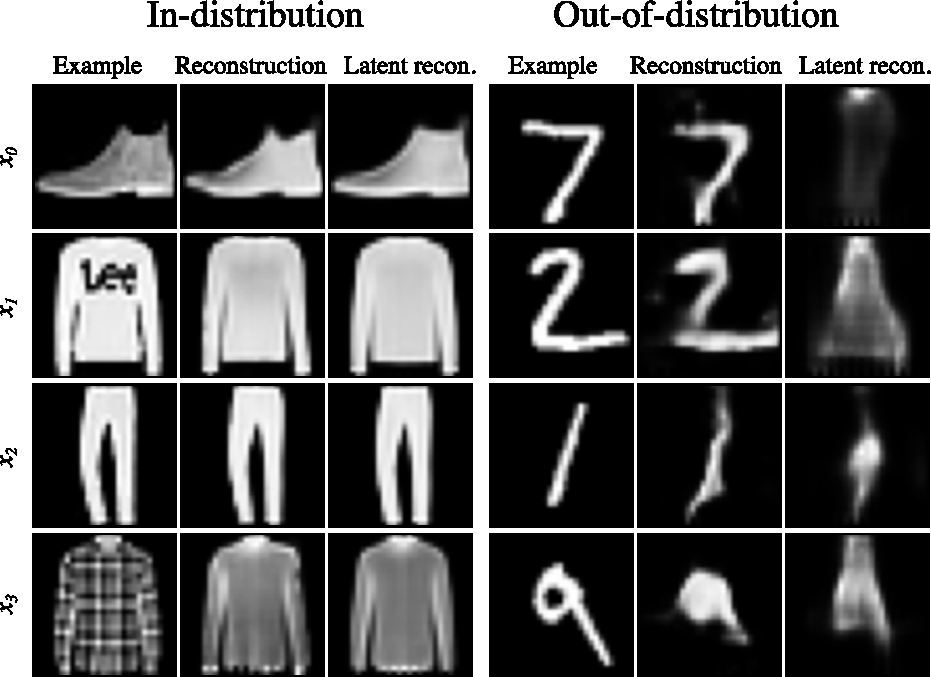
\includegraphics[width=0.7\columnwidth]{paper_hierarchical/reconstructions-front-page-4-samples-2-recons2.pdf}
    \caption[Reconstructions of a hierarchical VAE trained on FashionMNIST.]{%
        Reconstructions using a hierarchical VAE trained on FashionMNIST.
        Reconstruction quality of OOD data is comparable to in-distribution data, resulting in high likelihoods and poor OOD discrimination.
        By sampling the $k$ bottom-most latent variables from the conditional prior distribution $p(\zb_{\geq l}|\zb_{>l})$ (latent reconstructions) instead of the approximate posterior $q(\zb_{>l}|\zb_{<l})$, the model reconstructs from the training distribution resulting in lower $p(\xb|\zb)$ for OOD data.
    }
    \label{fig_hierarchical:reconstructions-fashionmnist}
\end{figure}
% First paragraph: Explains why OOD detection is important in a broad perspective
The reliability and safety of machine learning systems applied in the real-world is contingent on the ability to detect when an input is different from the training distribution. %, an anomaly.
Supervised classifiers built as deep neural networks are well-known to misclassify such \textit{out-of-distribution} (OOD) inputs to known classes with high confidence \cite{goodfellow_explaining_2015, nguyen_deep_2015}.
Several approaches have been suggested to equip deep classifiers with OOD detection capabilities \cite{hendrycks_baseline_2017, lakshminarayanan_simple_2017, hendrycks_deep_2019, devries_learning_2018}.
% However, such methods are inherently supervised and require in-distribution labels or examples of OOD data from an a priori known distribution which limit their applicability.
But, such methods are inherently supervised and require in-distribution labels or examples of OOD data limiting their applicability and generality.

% Second paragraph: Outline deep generative modeling approach and their failure
Unsupervised generative models that estimate an explicit likelihood should understand what it means to be in- and out-of-distribution without requiring labels or examples of OOD data.
By directly modeling the training distribution, such models are expected to assign low likelihoods to OOD data as it originates from regions of little or no support under the learned density \cite{bishop_novelty_1994}.
Recent advances in deep generative models \cite{kingma_autoencoding_2014, rezende_stochastic_2014, oord_pixel_2016, salimans_pixelcnn_2017, kingma_glow_2018} have enabled learning high quality generative models on complex data such as natural images, sequences including audio \cite{oord_wavenet_2016} and graphs \cite{kipf_variational_2016}.
However, recent observations have brought into question the quality of the learned density estimates by showing that they often assign higher likelihoods to OOD data than to in-distribution data \cite{nalisnick_deep_2019, choi_waic_2019}.
Many complex data distributions can be explained to a large degree by low-level features, e.g. edges in images.
However, such features do not explain high-level semantics of the data and may inhibit OOD detection \cite{ren_likelihood_2019, nalisnick_deep_2019}

\textbf{In this paper}, we examine the failure cases of deep generative models on OOD detection tasks within the context of hierarchical VAEs, and make the following contributions:
\begin{itemize}
    \item[(i)] We provide evidence that the root cause of OOD failures is that learned low-level features generalize well across datasets and dominate the estimated likelihoods.
    \item[(ii)] We then propose a fast, scalable, and fully unsupervised likelihood-ratio score for OOD detection that is explicitly developed to ensure that data should be in-distribution across all feature levels, which prevents the low-level features from dominating.
    \item[(iii)] With the likelihood-ratio score, we demonstrate state-of-the-art performance across a wide range of known OOD failure cases.
\end{itemize}


\section{Why does OOD detection fail?}\label{sec_paper_hierarchical:why-does-ood-fail}
\begin{figure}[t]
    \centering
    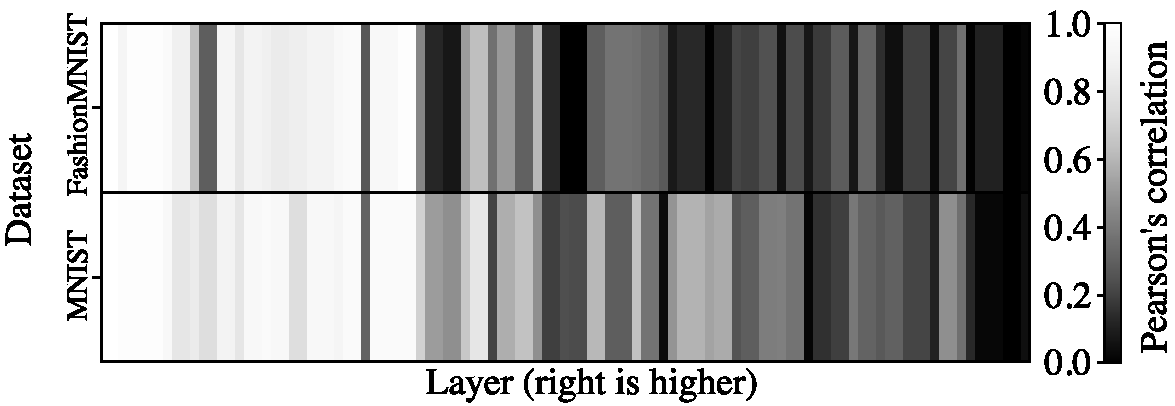
\includegraphics[width=1\columnwidth]{paper_hierarchical/feature-correlation-heatmap2.pdf}
    \vspace{0mm}
    \caption[Absolute correlations between data representations in all layers of the inference network of a hierarchical VAE trained on FashionMNIST and of another trained on MNIST.]{
    Absolute correlations between data representations in all layers of the inference network of a hierarchical VAE trained on FashionMNIST and of another trained on MNIST.
    We compute the correlation between the representations of the two different models given the same data, FashionMNIST (top) and MNIST (bottom).
    %We reduce the representations to a single number by summing over all dimensions and compute the correlation between these numbers for 256 examples.
    %To reduce de-correlation due to the stochastic latent variables, we encode using the mode of the approximate posterior distributions.
    }
    \vspace{0mm}
    \label{fig_hierarchical:correlations-heatmap}
\end{figure}

The inability to detect out-of-distribution data with deep generative models is surprising.
Before the advent of deep generative models, this was not considered a major issue for probabilistic models \cite{bishop_novelty_1994}.
Is the failure due to model pathologies or something different?

Deep learning models are generally believed to form hierarchies of representations that range from low-level features to more conceptual ones related to semantics \cite{bengio_representation_2013}.
This has also been observed within deep generative models \cite{maaloe_biva_2019, child_very_2021}.
%Recent research \cite{maaloe_biva_2019, child_very_2021, vahdat_nvae_2020}, has shown that deep latent variable models are able to learn rich hierarchical representations with increasing levels of abstraction and global structure towards the top of the hierarchy.
For image data there is a trend that the low-level features are quite similar across models (edge detectors, etc.). This raises the question to what extend such features are relevant when detecting OOD data, also suggested  by \cite{nalisnick_deep_2019} and examined for Glow and PixelCNN in \cite{schirrmeister_understanding_2020}.
To investigate, we train two hierarchical VAEs (\cref{sec_paper_hierarchical:background-hie-VAE}) on FashionMNIST and MNIST, respectively, and compute the between-models correlation of the extracted features of in-distribution data and OOD data.
The result appears in \cref{fig_hierarchical:correlations-heatmap}.
We observe that features extracted in the early layers (low-level features) correlate strongly between the two models, and that this correlation drops as we get into later layers.
This suggests that low-level features do not carry much information for OOD detection.

To shed further light on the impact of semantic versus low-level features, we look at model reconstructions of images with a hierarchical VAE (\cref{fig_hierarchical:biva-reconstructions-celeba}).
To study the feature hierarchy, we replace the inference distribution with the corresponding conditional prior in the first layers of the model to see what information is lost.
We observe that as more layers rely on the prior, more details are lost.
Sunglasses, which are uncommon, are first replaced by more common glasses, and then finally disappear.
%Likewise, a long-haired man eventually becomes woman.
This suggests that as we fall back to the conditional priors of each layer, we are pushed closer to local modes of the modeled distribution.

\begin{figure}[t]
    \centering
    %\vspace{0.17cm}
    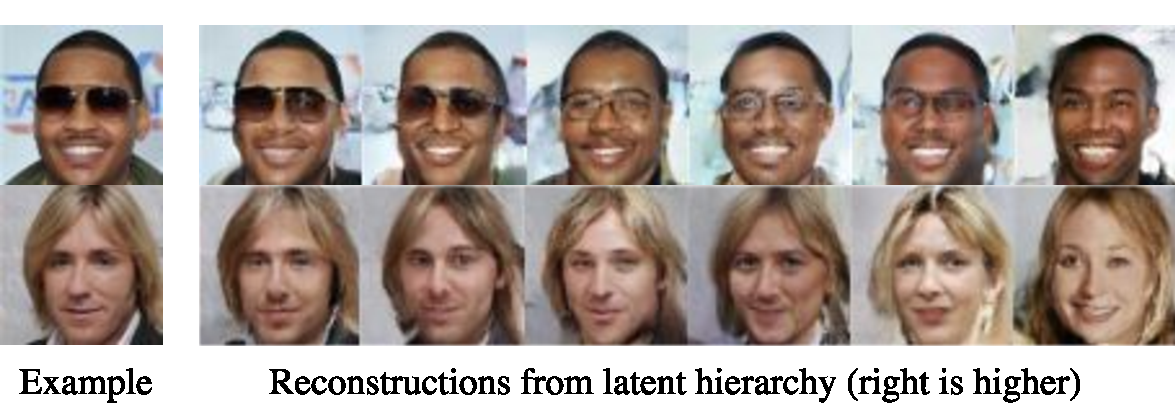
\includegraphics[width=1\columnwidth]{paper_hierarchical/biva_reconstructions.pdf}
    % https://docs.google.com/drawings/d/1UXdA3c18Oek9_env1vEB9mqOAHZ-tu0ijWmvqmapWCk/edit?usp=sharing
    \vspace{0mm}
    \caption[Reconstructions of in-distribution data (CelebA) of the BIVA model using higher latent variables.]{Reconstructions of in-distribution data (CelebA) of the BIVA model using higher latent variables  \cite{maaloe_biva_2019}.
    The higher the latent variable, the more the reconstructions fall into the mode of the learned distribution.
    It is more common to wear regular glasses than sunglasses but most common not to wear glasses at all.
    A man with long hair collapses into the mode of the more common long-haired woman.}
    \vspace{0mm}
    \label{fig_hierarchical:biva-reconstructions-celeba}
\end{figure}
Finally, we look at reconstructions of out-of-distribution data.
\cref{fig_hierarchical:reconstructions-fashionmnist} illustrates that MNIST data is surprisingly well reconstructed by a hierarchical VAE trained on FashionMNIST.
Similar results have been found elsewhere \cite{xiao_likelihood_2020}.
We repeat the previous experiment and replace inference distributions by their corresponding conditional prior, and now observe that reconstructions from higher latent layers become increasingly similar to the data on which the model was trained.
The reliance on conditional priors seems to prevent accurate reconstruction of out-of-distribution data.
Some details are lost on in-distribution data too, but the distinction between that and out-of-distribution data becomes more clear.

\textbf{These observations lead to our main hypothesis.}
The lowest latent variables in a hierarchical VAE learn generic features that can describe a wide range of data.
This enables the model to achieve high rates of compression and high likelihoods, even on out-of-distribution data as long as the learned low-level features are appropriate.
We further suggest that OOD data are in-distribution with respect to these low-level features, but not with respect to semantic ones.

\vspace{0cm}
\section{Background and related work}

\subsection{Variational autoencoders}
The variational autoencoder (VAE) \cite{kingma_autoencoding_2014, rezende_stochastic_2014} is a framework for constructing deep generative models defined by an observed variable $\mathbf{x}$ and a stochastic latent variable $\mathbf{z}$.
Typically, a neural network with parameters $\thetab$ is chosen to parameterize the generative distribution $p_\thetab(\xb,\zb)=p_\thetab(\xb|\zb)p(\zb)$, where the prior $p(\zb)$ is commonly a standard Gaussian $\mathcal{N}(\0, \Ib)$.
The true posterior $p(\zb|\xb)$ is generally not analytically tractable and is approximated by a variational distribution $q_\phib(\zb|\xb)$ parameterized via another neural network with parameters $\phib$. The approximate posterior $q_\phib(\zb|\xb)$ is most often  a diagonal covariance Gaussian.
The model parameters $\thetab$ and variational parameters $\phib$ are jointly optimized by maximizing the \textit{evidence lower bound} (ELBO),
\begin{equation}\label{eq_hierarchical:elbo}
    \log p_\thetab(\xb) \geq \mathbb{E}_{q_\phib(\zb|\xb)} \left[ \log \frac{p_\thetab(\xb,\zb)}{q_\phib(\zb|\xb)} \right] \equiv \mathcal{L}(\xb; \thetab, \phib)\ .
\end{equation}
For brevity, we will denote $\mathcal{L}(\xb; \thetab, \phib)$ as $\mathcal{L}(\xb)$ or $\mathcal{L}$. The reparameterization trick is used to backpropagate gradients through the stochastic latent variables with low variance.

The VAE is defined with a single latent variable which limits the ability to learn a high likelihood representation of complex input distributions, e.g.\ natural images.
There exists a few complementary approaches to make the VAE more flexible: (i) model a more expressive variational distribution $q_\phib(\zb|\xb)$ or prior distribution $p_\thetab(\zb)$ \cite{rezende_variational_2015, kingma_improved_2016}, (ii) model a more expressive posterior distribution $p_\thetab(\xb|\zb)$ e.g. with a autoregressive decoder \cite{oord_conditional_2016} and (iii) learn a deeper hierarchy of latent variables \cite{burda_importance_2016, sonderby_ladder_2016}.
Here, we focus on the latter.


\subsection{Hierarchical variational autoencoders}\label{sec_paper_hierarchical:background-hie-VAE}
Hierarchical VAEs are a family of probabilistic latent variable models which extends the basic VAE by introducing a hierarchy of $L$ latent variables $\zb=\zb_1, \dots, \zb_L$.
The most common generative model is defined from the top down as $p_\thetab(\xb|\zb)=p(\xb|\zb_1)p_\thetab(\zb_1|\zb_2)\cdots p_\thetab(\zb_{L-1}|\zb_L)$.
The inference model can then be defined in two ways respectively referred to as \textit{bottom-up} \cite{burda_importance_2016}
\begin{equation}
    %q_\phib(\zb|\xb)=q_\phib(\zb_1|\xb)q_\phib(\zb_2|\zb_1)\cdots q_\phib(\zb_L|\zb_{L-1})
    q_\phib(\zb|\xb) = q_\phib(\zb_1|\xb)\textstyle\prod_{i=2}^{L} q_\phib(\zb_i|\zb_{i-1})
\end{equation}
and \textit{top-down} \cite{sonderby_ladder_2016}
\begin{equation}
    % q_\phib(\zb|\xb)=q_\phib(\zb_{L}|\xb)q_\phib(\zb_{L-1}|\zb_L)\cdots q_\phib(\zb_2|\zb_1),
    q_\phib(\zb|\xb) = q_\phib(\zb_L|\xb)\textstyle\prod_{i=L-1}^{1} q_\phib(\zb_{i}|\zb_{i+1}) \ .
\end{equation}
Regardless of the choice of inference model, a hierarchical VAE is still trained using the ELBO \cref{eq_hierarchical:elbo}.

Until recently, hierarchical VAEs gave inferior likelihoods compared to state-of-the-art autoregressive \cite{ho_flow_2019} and flow-based models \cite{salimans_pixelcnn_2017}.
This was changed by \textcite{maaloe_biva_2019}, \textcite{vahdat_nvae_2020}, and \textcite{child_very_2021}, which introduced complementary methods to extend the number of latent variables to a very deep hierarchy resulting in state-of-the-art likelihood performance.

In this paper we employ a simple hierarchical VAE with bottom-up inference paths and the more powerful BIVA variant with a bidirectional (top-down and bottom-up) inference model \cite{maaloe_biva_2019}. We employ skip connections between latent variables but omit them for brevity.


\subsection{Out-of-distribution detection}\label{sec_paper_hierarchical:background-ood-detection}
% Intro to alternative scores
So far, no reliable direct likelihood-based method has been found for fully unsupervised deep generative model OOD detection.
A major line of work considers developing new scores that are more reliable than the likelihood.
This includes the \textit{typicality} test presented by \textcite{nalisnick_detecting_2019} which is an OOD detection test based on the typicality of a batch of potentially OOD examples.
This approach however requires a batch of examples from the same class (OOD or not) which limits its practical applicability.
In \textcite{ren_likelihood_2019}, the \textit{likelihood ratio} between a primary model and a background model was shown to be an effective score for OOD detection.
However, to train the background model, the in-distribution data is perturbed via a data augmentation technique that is designed with knowledge about the confounding factors between the in-distribution data and the OOD data. Furthermore, it is tuned towards high performance on a known OOD dataset.
\textcite{serra_input_2020} take a similar approach and attribute the failure to detect OOD data to the high influence of the input complexity on the likelihood and choose a generic lossless compression algorithm as the background model.
Although this method gives good results, no single best choice of compression algorithm exists for all types of OOD data, and any particular choice encodes prior knowledge about the data into the detection method.
Both these methods can be seen as correcting for low-level features of the OOD data being assigned high model likelihood by using a second model focused exclusively on these features.

Similar to these methods, the majority of the approaches to OOD detection make assumptions about the nature of the OOD data.
The assumptions encompass using labels on the in-distribution data \cite{hendrycks_baseline_2017, liang_enhancing_2018, alemi_uncertainty_2018, lee_simple_2018, lakshminarayanan_simple_2017}, examples of OOD data \cite{hendrycks_deep_2019}, augmenting in-distribution data to mimic it \cite{ren_likelihood_2019}, or assuming a certain data type \cite{serra_input_2020}.
Any of these assumptions encode implicit biases into the model about the attributes of OOD data which, in turn, might impair performance on truly unknown data examples (unknown unknowns).

% Introduce the contrast to results with VAEs
While some of these methods achieve very good results on OOD detection with autoregressive models \cite{oord_pixel_2016, salimans_pixelcnn_2017} and invertible flow-based models \cite{kingma_glow_2018}, it was recently shown that they can be much less effective for VAEs \cite{xiao_likelihood_2020} highlighting the need for a more reliable OOD score for VAEs.
Although VAEs have the same failure cases as autoregressive and flow-based models, the caveat is that the difference in the likelihood is generally not as big and reconstructions of OOD can be surprisingly good \cite{xiao_likelihood_2020}.
\textcite{xiao_likelihood_2020} alleviate this by refitting the inference network, as previously proposed by \textcite{cremer_inference_2018, mattei_refit_2018}, to a potentially OOD example and measuring the so-called \textit{likelihood regret}.
However, refitting the inference network can be computationally expensive, especially for the large hierarchical VAEs that are used to model complex data \cite{maaloe_biva_2019, vahdat_nvae_2020, child_very_2021}. Furthermore, this scales poorly to large amounts of potentially OOD examples as the optimization is done per example.

A few methods have approached OOD detection in a completely unsupervised fashion \cite{maaloe_biva_2019, choi_waic_2019, xiao_likelihood_2020}.
The work of \textcite{maaloe_biva_2019} is the most related to ours. They introduce BIVA, a deep hierarchy of stochastic latent variables with a top-down and bottom-up inference model and achieve state-of-the-art likelihood scores. 
They also provide early results indicative that a looser likelihood bound may have value in OOD detection.
In this paper, we provide an explanation of those results, and significantly improve upon them.


\section{OOD detection with hierarchical VAEs}
\subsection{A bound for semantic OOD detection}
If the lowest latent variable in the VAE hierarchy codes for a large part of the low-level features required to reconstruct the input with high accuracy, as exemplified in \cref{fig_hierarchical:reconstructions-fashionmnist}-\ref{fig_hierarchical:biva-reconstructions-celeba}, then $p_\thetab(\xb|\zb_1)$ will be high for both in- and out-of-distribution data.
Hence, any OOD detection capabilities based on the ELBO $\mathcal{L} = \mathbb{E}_{q_\phib(\zb|\xb)}[\log p_\thetab(\xb|\zb_1)] - D_{\mathrm{KL}}( q_\phib(\zb|\xb) || p(\zb))$ from \cref{eq_hierarchical:elbo} relies on the KL-term for OOD detection. For a bottom-up hierarchical VAE, the KL-term $D_{\mathrm{KL}}( q_\phib(\zb|\xb) || p(\zb))$ can be expressed by a hierarchical sum% over the hierarchy
% \begin{multline}
%     \mathcal{L}(\xb) =  \mathbb{E}_{q_\phib(\zb|\xb)} \Big[ \log p_\thetab(\xb|\zb_1) \\
%                      + \textstyle\sum_{i=1}^{L-1} \log \frac{p_\thetab(\zb_i|\zb_{i+1})}{q_\phib(\zb_i|\zb_{i-1})} 
%                      + \log \frac{p_\thetab(\zb_L)}{q_\phib(\zb_L|\zb_{L-1})} \Big] .
% \end{multline}
% \begin{multline}
%     D_{\mathrm{KL}}( q(\zb|\xb) || p(\zb)) = \\
%     \mathbb{E}_{q_\phib(\zb|\xb)} \Big[ \textstyle\sum_{i=1}^{L-1} \log \frac{p_\thetab(\zb_i|\zb_{i+1})}{q_\phib(\zb_i|\zb_{i-1})} + \log \frac{p_\thetab(\zb_L)}{q_\phib(\zb_L|\zb_{L-1})} \Big] .
% \end{multline}
\begin{equation}
    \mathbb{E}_{q_\phib(\zb|\xb)} \Big[ \textstyle\sum_{i=1}^{L-1} \log \frac{p_\thetab(\zb_i|\zb_{i+1})}{q_\phib(\zb_i|\zb_{i-1})} + \log \frac{p_\thetab(\zb_L)}{q_\phib(\zb_L|\zb_{L-1})} \Big] \ .
\end{equation}
In general, the absolute log-ratios grow with $\mathrm{dim}(\zb_i)$ as the individual log probability terms are computed by summing over the dimensionality of $\zb_i$.
This means that the value of the KL-term is dominated by terms where $\zb_i$ is high-dimensional. We refer to Appendix C for a more detailed argument.
Since hierarchical VAEs are generally constructed with a bottleneck type structure, the terms corresponding to latent variables towards the top of the hierarchy will have a vanishing influence on the value of the KL-term.
However, as the semantic information most relevant for OOD detection has a tendency to be represented in the top-most latent variables, this makes OOD detection using the regular ELBO difficult, even for state-of-the-art models.
This behavior has also been reported by \textcite{xiao_likelihood_2020}.

To shift the ELBO from primarily being based on the approximate posterior of the lowest latent variables to instead focus on the conditional prior, \textcite{maaloe_biva_2019} introduced slightly different likelihood lower bound defined as
\begin{equation}\label{eq_hierarchical:biva->k}
    \mathcal{L}^{>k} = \mathbb{E}_{p_\thetab(\zb_{\leq k}|\zb_{>k}) q_\phib(\zb_{>k}|\xb)} \left[ \log \frac{p_\thetab(\xb|\zb)p_\thetab(\zb_{>k})}{q_\phib(\zb_{>k}|\xb)} \right]
\end{equation}
where $k\in\{0,1,\dots,L\}$ (see Appendix for the derivation).
We note that $\mathcal{L}^{>0}$ is the regular ELBO (\cref{eq_hierarchical:elbo}) and that empirically we always observe that $\mathcal{L}\geq\mathcal{L}^{>k} \, \forall \, k$ although this need not hold in general.
The core idea behind this variation on the ELBO is to sample the $k$ lowest latent variables from the conditional prior $\zb_1,\dots,\zb_l \sim p_\thetab(\zb_{\leq k}|\zb_{>k})$ and only the $L-k$ highest from the approximate posterior $\zb_{k+1},\dots,\zb_L \sim q_\phib(\zb_{>k}|\xb)$.
Importantly, this has the effect that the data likelihood $p(\xb|\zb)$ is dependent on the approximate posterior through a latent variable $\zb_{k+1}$ different from $\zb_1$ for all $k \geq 1$.
Thereby, the likelihood can be evaluated with a reconstruction from each of the latent variables $\zb_k$ of the hierarchical VAE.
Hence, we can now test how well the input $\xb$ is reconstructed from each latent variable.
The notation $\mathcal{L}^{>k}$ highlights that for latent variables $\zb_{>k}$, the bound is the regular ELBO while for the latent variables $\zb_{\leq k}$, the bound is evaluated using the (conditional) prior rather than the approximate posterior as the proposal distribution.


\subsection{A likelihood-ratio score for all feature levels}
While the $\mathcal{L}^{>k}$ bound provides a score for performing semantic OOD detection, it still relies on the data space likelihood function (see equation \cref{eq_hierarchical:likelihoods-as-exact} below), which is known to be problematic for OOD detection (\cref{sec_paper_hierarchical:background-ood-detection}). To alleviate this, we phrase OOD detection as a likelihood ratio test of being \emph{semantically} in-distribution.
A standard likelihood ratio test \cite{buse_likelihood_1982} suggests to consider the ratio between the associated likelihoods, which we can approximate on a log-scale by the corresponding lower bounds $\mathcal{L}$ and $\mathcal{L}^{>k}$,
\begin{equation}\label{eq_hierarchical:llr-as-difference-in-likelihoods}
    % LLR = - 2 log(L0 / L1)
    % where L0 < L1 so log(L0 / L1) < 0 and LLR > 0
    % LLR = 2 log(L1 / L0)
    %     = 2 (log(L1) - log(L0))
    %     = 2 (ELBO - L^{>k})  % LLR^{>a,>b} where a=0
    % L1 = ELBO
    % L0 = L^{>k}
    LLR^{>k}(\xb) = \mathcal{L}(\xb) - \mathcal{L}^{>k}(\xb) \ .
\end{equation}
%This likelihood ratio contrasts the ELBO with $\mathcal{L}^{>k}$ for a variable choice of $k$.
Since, empirically, $\mathcal{L}\geq\mathcal{L}^{>k}$, the ratio is always positive as is standard for likelihood ratio tests.
A low value of $LLR^{>k}(\xb)$ means that the ELBO and $\mathcal{L}^{>k}$ are almost equally tight for the data.
On the contrary, a high value indicates that $\mathcal{L}^{>k}$ is looser on the data than the ELBO; hence, the data may be OOD.


We can gather further insights about this score if we write the regular ELBO and the $\mathcal{L}^{>k}$ bounds in the exact form that includes the intractable KL-divergence between the approximate and true posteriors,
\begin{align}
    \mathcal{L}      &= \log p_\thetab(\xb) - D_{\mathrm{KL}}\left( q_\phib(\zb|\xb) || p_\thetab(\zb|\xb)\right), \label{eq_hierarchical:likelihoods-as-exact} \\ 
    \mathcal{L}^{>k} &= \log p_\thetab(\xb) - D_{\mathrm{KL}}\left( p_\thetab(\zb_{\leq k }|\zb_{>k}) q_\phib(\zb_{>k}|\xb) || p_\thetab(\zb|\xb)\right) \nonumber \ .
\end{align}
Subtracting these cancel out the two data likelihood terms $\log p_\thetab(\xb)$ and only the KL-divergences from the approximate to the true posterior remain,
\begin{align}
    LLR^{>k}(\xb) &= - D_{\mathrm{KL}}\left( q_\phib(\zb|\xb) || p_\thetab(\zb|\xb)\right) \\
                 &\quad + D_{\mathrm{KL}}\left( p_\thetab(\zb_{\leq k}|\zb_{>k}) q_\phib(\zb_{>k}|\xb) || p_\thetab(\zb|\xb)\right) \ . \notag
\end{align}\label{eq_hierarchical:llr-as-kls}

Hence, it is clear that compared to the likelihood bound $\mathcal{L}^{>k}$, this likelihood-ratio measures divergence exclusively in the latent space whereas $\mathcal{L}^{>k}$ includes the $\log p_\thetab(\xb)$ term similar to the ELBO.
Therefore, the $LLR^{>k}$ score should be an improved method for semantic OOD detection compared to $\mathcal{L}^{>k}$.
Now, it can be noted that if we replace the regular ELBO, $\mathcal{L}$, in \cref{eq_hierarchical:likelihoods-as-exact} with the strictly tighter importance weighted bound \cite{burda_importance_2016},
\begin{equation}
    \mathcal{L}_{S} = \mathbb{E}_{q(\zb|\xb)}\left[ \log \frac{1}{N} \sum_{s=1}^{S} \frac{p(\xb, \zb^{(s)})}{q(\zb^{(s)}|\xb)} \right] \ , \label{eq_hierarchical:iw-bound}
\end{equation}
then, in the limit $S\rightarrow\infty$, we have $\mathcal{L}_{S} \rightarrow \log p_\thetab(\xb)$ and the likelihood ratio reduces to
\begin{equation}
    LLR^{>k}_{S}(\xb) \rightarrow D_{\mathrm{KL}}( p(\zb_{\leq k}|\zb_{>k}) q(\zb_{>k}|\xb) || p(\zb|\xb))
\end{equation}\label{eq_hierarchical:llr-as-kls-iwae-reduced}
which, in practice, is well-approximated for a finite $S$. We expect this importance weighted likelihood ratio to monotonically improve upon the one in \cref{eq_hierarchical:llr-as-kls} as $S$ increases and the KL-divergence in the regular ELBO that contains terms for which $\zb_i$ is high-dimensional goes to zero.


Since the scores in \cref{eq_hierarchical:llr-as-kls,eq_hierarchical:llr-as-kls-iwae-reduced} are estimated by sampling their estimators are stochastic objects with nonzero variance.
We note that $\text{Var}(\widehat{LLR}^{>k}) = \text{Var}(\hat{\mathcal{L}}) + \text{Var}(\hat{\mathcal{L}}^{>k}) - 2\, \text{Cov}(\hat{\mathcal{L}}, \hat{\mathcal{L}}^{>k})$.
Since $\log p_\thetab(\xb)$ and part of the KL divergence are identical in the expressions of $\mathcal{L}$ and $\mathcal{L}^{>k}$ we expect $\text{Cov}(\hat{\mathcal{L}}, \hat{\mathcal{L}}^{>k})$ to be positive which reduces the total variance. 
Empirical results indeed show that $\text{Var}(\widehat{LLR}^{>k})$ is larger than $\text{Var}(\hat{\mathcal{L}})$ but smaller than $\text{Var}(\hat{\mathcal{L}}^{>k})$.
%Whether this decreases the variance to below the variance of any of the two bounds, we do not know, and we believe it to be difficult to verify mathematically.
Nevertheless, the variance of the estimators is guaranteed to go to zero as the number of samples is increased.

The OOD scores considered in this research all assume that what discriminates an out-of-distribution from an in-distribution data point are semantic, high-level features. Clearly, if this is not the case and the difference instead lies in low-level statistics, the scores would likely fail. We hypothesize that a complementary bound to \cref{eq_hierarchical:biva->k}, $\mathcal{L}^{<l}$ described in Appendix E, might be useful in these cases, but leave further examination to future work.


\section{Experimental setup}

\paragraph{Tasks} We follow existing literature \cite{nalisnick_deep_2019, hendrycks_deep_2019} and evaluate our method by setting up OOD detection tasks from FashionMNIST \cite{xiao_fashionmnist_2017} to MNIST \cite{lecun_gradientbased_1998} and from CIFAR10 \cite{krizhevsky_learning_2009} to SVHN \cite{netzer_reading_2011}.
For each experiment we train our model on the train split of the former dataset and test its ability to recognize the test split of the latter dataset as OOD from the test split of the former dataset.
We use the standard train/test splits for the datasets.
More details on the datasets can be found in the Appendix.


% Our model
%\begin{wrapfigure}{R}{0.5\columnwidth}
% \begin{SCfigure}[50][t!]
\begin{figure}[t]
    %\begin{figure}
    \centering
    \resizebox{0.25\textwidth}{!}{
    \tikz{
        % inference
        % nodes
        \node[obs] (x_inf) {$\xb$};%
        \node[latent,above=.75cm of x_inf](z1_inf){$\zb_1$}; %
        \node[latent,above=.75cm of z1_inf](z2_inf){$\zb_2$}; %
        % \node[latent,above=.75cm of z2_inf](z3_inf){$\zb_3$}; %
        \node[above=of z2_inf, yshift=-1.cm] (phi) {$q_\phib(\zb|\xb)$}; 
        
        % edges
        \edge[]{x_inf}{z1_inf};
        \edge[]{z1_inf}{z2_inf};
        % \edge[]{z2_inf}{z3_inf};
        \edge[dashed, bend left]{x_inf}{z2_inf};
        % \edge[dashed, bend left]{x_inf}{z3_inf};
        
        % generative
        % nodes$
        \node[obs,right=0.75cm of x_inf] (x_gen) {$\xb$};%
        \node[latent,above=.75cm of x_gen](z1_gen){$\zb_1$}; %
        \node[latent,above=.75cm of z1_gen](z2_gen){$\zb_2$}; %
        % \node[latent,above=.75cm of z2_gen](z3_gen){$\zb_3$}; %
        \node[above=of z2_gen, yshift=-1.cm] (theta) {$p_\thetab(\xb,\zb)$}; 
        
        % edges
        % \edge[]{z3_gen}{z2_gen};
        \edge[]{z2_gen}{z1_gen};
        \edge[]{z1_gen}{x_gen};
        \edge[dashed, bend left]{z2_gen}{x_gen};
        % \edge[dashed, bend left]{z3_gen}{x_gen};
    }
    }
    \caption[Inference and generative models for a bottom-up hierarchical VAEs.]{The inference and generative models, $q_\phib$ and $p_\thetab$, for an $L=2$ layered bottom-up hierarchical VAE as the one used in our experiments.
    Dashed lines indicate deterministic skip connections which are employed in both networks. Skip connections are found to be useful for optimizing latent variable models \cite{dieng_avoiding_2019, maaloe_biva_2019}.}
    \label{fig_hierarchical:hvae-graphical-model}
    % \end{figure}
%\end{wrapfigure}
% \end{SCfigure}
\end{figure}


\paragraph{Models} For each OOD task, we train a simple bottom-up hierarchical VAE with $L$ stochastic layers which we will refer to as ``HVAE''.
To alleviate posterior collapse we include skip-connections that connect $\zb_i$ to $\zb_{i+2}$ for $i\in\{0, L-2\}$ and $\zb_0\equiv\xb$ in both the inference and generative models \cite{dieng_avoiding_2019} and employ the \textit{free bits} scheme with $\lambda=2$ \cite{kingma_improved_2016}.
We use weight-normalization \cite{salimans_weight_2016} on all weights and residual networks in the deterministic paths. 
A graphical representation of this model can be seen in \cref{fig_hierarchical:hvae-graphical-model}.
We use a Bernoulli output distribution for FashionMNIST/MNIST and a discretized mixture of logistics output distribution \cite{salimans_pixelcnn_2017} for CIFAR10/SVHN.
We use $L=3$ for grey-scale images and $L=4$ for natural images.
% For CIFAR/SVHN, we also train a BIVA model \cite{maaloe_biva_2019} with $L=10$ and similar configuration as used by the original paper\footnote{Code available at \url{github.com/larsmaaloee/BIVA} and \url{github.com/vlievin/biva-pytorch}}.
Full model details are in the Appendix.


% Baselines
\paragraph{Baselines} We group baselines into those that use prior knowledge about OOD data, ones that use labels associated with the in-distribution data and purely unsupervised approaches that do not make such assumptions.
Our method falls into the latter category.
For more information on each baseline, we refer to the original literature.


% Metrics and Evaluation
\paragraph{Evaluation} Following previous work \cite{hendrycks_baseline_2017, hendrycks_deep_2019, alemi_uncertainty_2018, ren_likelihood_2019, choi_waic_2019} we use the threshold-independent evaluation metrics of Area Under the Receiver Operator Characteristic (AUROC$\uparrow$), Area Under the Precision Recall Curve (AUPRC$\uparrow$) and False Positive Rate at 80\% true positive rate (FPR80$\downarrow$) where the arrow indicates the direction of improvement.
Note that these metrics are only computable given examples of OOD data but faced with truly OOD data (unknown unknowns), there are many ways to select thresholds to use in practice e.g.\ as the one that yields a specific tolerable false positive rate on the in-distribution test data.
To compute the metrics, we use an equal number of samples from the in-distribution and OOD datasets by including all examples in the smallest of the two sets and randomly sampling equally many from the larger. We compute the $LLR^{>k}$ score with one and $S$ importance samples denoted by $LLR^{>k}_S$.

% The value of k
\paragraph{Selection of $k$} To determine whether an example is OOD in practice, the value of $LLR^{>k}$ is computed on the in-distribution test set for all $k$ and the resulting empirical distribution is used as reference.
If for any value of $k$, the $LLR^{>k}$ score of a new input differs significantly from the empirical distribution, it is regarded OOD.
If it differs for multiple values of $k$, the value for which it differs the most is selected.
In our experiments, we consider an entire dataset at a time and report the results of $LLR^{>k}$ with the value of $k$ that yielded the highest AUROC$\uparrow$ for that dataset in a threshold-free manner.
In practice, slightly better performance may be achieved by choosing $k$ per example.
This would not exclude the use of batching in our method, since $LLR^{>k}$ is computed after the forward pass.


\section{Results}

The likelihoods for our trained models are in \cref{tab_hierarchical:bits-per-dim-ood} alongside baseline results for in-distribution and OOD data.
The main results of the paper on the OOD tasks can be seen along with comparisons to the baseline methods in \cref{tab_hierarchical:rocauc-ood}.
We note that for all our results, the value of the score ($\mathcal{L}^{>k}$ and $LLR^{>k}$) for the training and test splits of the in-distribution data was observed to have the same empirical distribution to within sampling error hence yielding an AUROC score of $\approx0.5$ as expected.
Results on additional commonly used datasets are found in Appendix G.


\begin{table}[t!]
    \centering
    \resizebox{0.8\columnwidth}{!}{%
    \begin{tabular}{lrrrrr}
        \toprule
         Method & Dataset & \multicolumn{4}{c}{Avg. bits/dim}\\
        %   & & $\log p(x)$ & $\mathcal{L}^{>k_1}$ & $\mathcal{L}^{>k_2}$ & $\mathcal{L}^{>k_3}$\\
          & & $\log p(x)$ & $\mathcal{L}^{>1}$ & $\mathcal{L}^{>2}$ & $\mathcal{L}^{>3}$\\
         \midrule
         \multicolumn{6}{c}{\textbf{Trained on FashionMNIST}} \\
         \midrule
         \multirow{2}{*}{Glow}
            & FashionMNIST & 2.96 & - & - & \\
            & MNIST & 1.83 & - & - & \\
         \multirow{2}{*}{HVAE (Ours)}
            & FashionMNIST & 0.420 & 0.476 & 0.579 & - \\
            & MNIST & 0.317 & 0.601 & 0.881 & - \\
         \midrule
         \multicolumn{6}{c}{\textbf{Trained on CIFAR10}} \\
         \midrule
         \multirow{2}{*}{Glow}
          & CIFAR10 & 3.46 & - & - & \\
          & SVHN & 2.39 & - & - & \\
         \multirow{2}{*}{HVAE (Ours)}
            & CIFAR10 & 3.74 & 17.8 & 54.3 & 75.7 \\  % log p(x) = 8010.03
            & SVHN & 2.62 & 10.2 & 64.0 & 93.9 \\
         \multirow{2}{*}{BIVA (Ours)}
          & CIFAR10 & 3.46 & 8.74 & 19.7 & 37.3 \\
          & SVHN & 2.35 & 6.62 & 25.1 & 59.0 \\
         \bottomrule
    \end{tabular}
    }
    \caption[Average bits per dimension of different datasets for generative models trained on FashionMNIST and CIFAR10.]{%
    Average bits per dimension of different datasets for models trained on FashionMNIST and CIFAR10.
    For the hierarchical models we include the $\mathcal{L}^{>k}$ bounds.
    The likelihoods of training and test splits of the in-distribution data are all cases close.
    Since we train on dynamically binarized FashionMNIST, our bits/dim are smaller than for Glow.
    As $k$ is increased for the $L^{>k}$ bound, the bound gets looser but the model eventually assigns higher likelihood to the in distribution data than to the OOD data.
    Glow refers to \textcite{kingma_glow_2018, nalisnick_deep_2019}.
    BIVA refers to our implementation of \textcite{maaloe_biva_2019}.}
    \label{tab_hierarchical:bits-per-dim-ood}
    \vspace{0mm}
\end{table}

\footnotetext{%
    \textcite{serra_input_2020} performs the best when high likelihoods are assigned to OOD data such that the overlap with in-distribution data is low.
    Performance is worse when the overlap is high, cf. \textcite[Table 1]{serra_input_2020}, as seen with complex images.}
\begin{table}[t!]
    \centering
    \resizebox*{!}{0.9\textheight}{%
    \begin{tabular}{lrrr}
        \toprule
         Method & AUROC$\uparrow$ & AUPRC$\uparrow$ & FPR80$\downarrow$ \\
         \midrule
         \multicolumn{4}{c}{\textbf{FashionMNIST (in) / MNIST (out)}} \\
         \midrule
         \multicolumn{4}{l}{\textbf{Use prior knowledge of OOD}} \\
Backgr. contrast. LR (PixelCNN) {\cite{ren_likelihood_2019}}               & $0.994$ & $0.993$ & $0.001$ \\
Backgr. contrast. LR (VAE) {\cite{choi_waic_2019}}                    & $0.924$ & - & - \\
Binary classifier {\cite{ren_likelihood_2019}}                              & $0.455$ & $0.505$ & $0.886$ \\ % 6
$p(\hat{y} | \xb)$ with OOD as noise class {\cite{ren_likelihood_2019}}     & $0.877$ & $0.871$ & $0.195$ \\ % 7
$p(\hat{y} | \xb)$ with calibration on OOD {\cite{ren_likelihood_2019}}     & $0.904$ & $0.895$ & $0.139$ \\ % 8
Input complexity ($S$, Glow) \cite{hendrycks_deep_2019}                    & $0.998$ & - & - \\
Input complexity ($S$, PixelCNN++) \cite{hendrycks_deep_2019}              & $0.967$ & - & - \\
         \multicolumn{4}{l}{\textbf{Use in-distribution data labels $y$}} \\
$p(\hat{y} | \xb)$ {\cite{ren_likelihood_2019, hendrycks_baseline_2017}}                        & $0.734$ & $0.702$ & $0.506$ \\
Entropy of $p(y | \xb)$ {\cite{ren_likelihood_2019}}                        & $0.746$ & $0.726$ & $0.448$ \\
ODIN {\cite{ren_likelihood_2019, liang_enhancing_2018}}                                       & $0.752$ & $0.763$ & $0.432$ \\
VIB \cite{alemi_uncertainty_2018, choi_waic_2019}                                          & $0.941$ & - & - \\
Mahalanobis distance, CNN {\cite{ren_likelihood_2019}}                     & $0.942$ & $0.928$ & $0.088$ \\
Mahalanobis distance, DenseNet {\cite{lee_simple_2018}}                & $0.986$ & - & - \\
Ensemble, 20 classifiers {\cite{ren_likelihood_2019, lakshminarayanan_simple_2017}}                  & $0.857$ & $0.849$ & $0.240$ \\
         \multicolumn{4}{l}{\textbf{No OOD-specific assumptions}} \\
         \multicolumn{4}{l}{\textit{- Ensembles}} \\
WAIC, 5 models, VAE {\cite{choi_waic_2019}}                          & $0.766$ & - & - \\
WAIC, 5 models, PixelCNN {\cite{ren_likelihood_2019}}                      & $0.221$ & $0.401$ & $0.911$ \\
        \multicolumn{4}{l}{\textit{- Not ensembles}} \\
Likelihood regret \cite{xiao_likelihood_2020}                               & $\mathbf{0.988}$ & - & - \\
$\mathcal{L}^{>0}$ + HVAE (ours)                    & $0.268$ & $0.363$ & $0.882$ \\
$\mathcal{L}^{>1}$ + HVAE (ours)                    & $0.593$ & $0.591$ & $0.658$ \\
$\mathcal{L}^{>2}$ + HVAE (ours)                    & $0.712$ & $0.750$ & $0.548$ \\
$LLR^{>1}$ + HVAE (ours)                            & $0.964$ & $0.961$ & $0.036$ \\
$LLR^{>1}_{250}$ + HVAE (ours)                      & $0.984$ & $\mathbf{0.984}$ & $\mathbf{0.013}$ \\
         \midrule
         \multicolumn{4}{c}{\textbf{CIFAR10 (in) / SVHN (out)}} \\
         \midrule
         \multicolumn{4}{l}{\textbf{Use prior knowledge of OOD}} \\
Backgr. contrast. LR (PixelCNN) {\cite{ren_likelihood_2019}}               & $0.930$ & $0.881$ & $0.066$ \\
Backgr. contrast. LR (VAE) {\cite{xiao_likelihood_2020}}                    & $0.265$ & - & - \\
Outlier exposure {\cite{hendrycks_deep_2019}}                              & $0.984$ & - & - \\
Input complexity ($S$, Glow) \cite{serra_input_2020}                   & $0.950$ & - & - \\
Input complexity ($S$, PixelCNN++) \cite{serra_input_2020}             & $0.929$ & - & - \\
Input complexity ($S$, HVAE) (Ours) \cite{serra_input_2020}\footnotemark & $0.833$ & $0.855$ & $0.344$ \\
         \multicolumn{4}{l}{\textbf{Use in-distribution data labels $y$}} \\
Mahalanobis distance {\cite{lee_simple_2018}}                          & $0.991$ & - & -  \\
         \multicolumn{4}{l}{\textbf{No OOD-specific assumptions}} \\
         \multicolumn{4}{l}{\textit{- Ensembles}} \\
WAIC, 5 models, Glow {\cite{choi_waic_2019}}                          & $1.000$ & - & - \\
WAIC, 5 models, PixelCNN {\cite{ren_likelihood_2019}}                      & $0.628$ & $0.616$ & $0.657$ \\
         \multicolumn{4}{l}{\textit{- Not ensembles}} \\
Likelihood regret \cite{xiao_likelihood_2020}                               & $0.875$ & - & - \\
$LLR^{>2}$ + HVAE (ours)                            & $0.811$ & $0.837$ & $0.394$ \\
$LLR^{>2}$ + BIVA (ours)                            & $\mathbf{0.891}$ & $\mathbf{0.875}$ & $\mathbf{0.172}$ \\
         \bottomrule
    \end{tabular}%
    }
    \caption[AUROC, AUPRC, and FPR80 of generative models for OOD detection (MNIST/FashionMNIST and SVHN/CIFAR10).]{%
        AUROC$\uparrow$, AUPRC$\uparrow$ and FPR80$\downarrow$ for OOD detection for a FashionMNIST model using scores on the FashionMNIST test set as reference. We bold the best results within the "No OOD-specific assumptions" group since we only compare directly to those.
        HVAE (ours) refers to our hierarchical bottom-up VAE.
        BIVA (ours) refers to our implementation of the hierarchical BIVA model \cite{maaloe_biva_2019}.
    }
    \label{tab_hierarchical:rocauc-ood}
\end{table}


\subsection{Likelihood-based OOD detection}
% \begin{sidewaysfigure}
\begin{figure}
    %\captionstyle{centerlast}
    \centering
    \begin{subfigure}[l]{0.48\columnwidth}
        \centering
        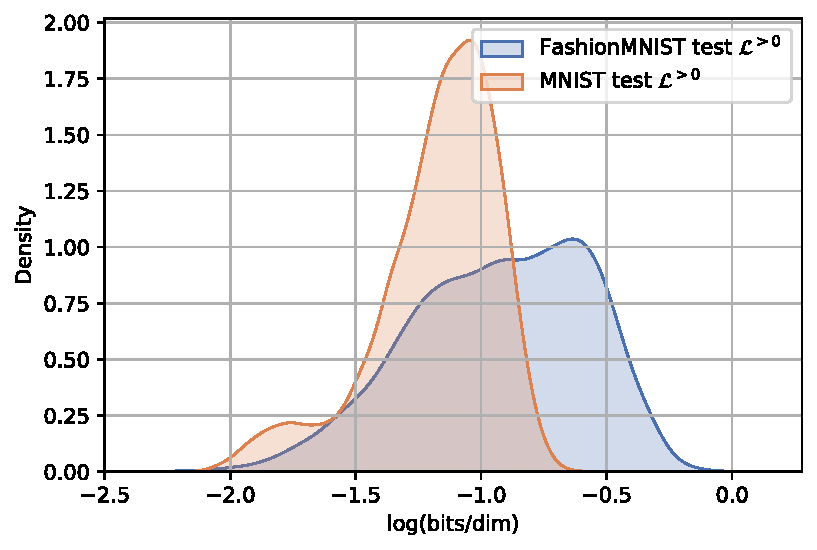
\includegraphics[width=1\columnwidth]{paper_hierarchical/densities-FashionMNIST-test-MNIST-test-bpp-k-0_sohau.pdf}
        \caption{}
        \label{fig_hierarchical:FMNIST-elbo-k0}
    \end{subfigure}
    % \hfill
    \begin{subfigure}[c]{0.48\columnwidth}
        \centering
        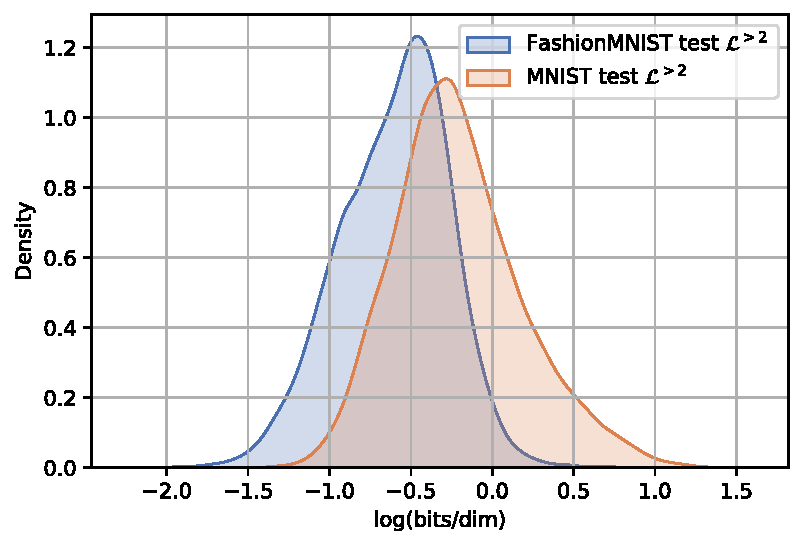
\includegraphics[width=1\columnwidth]{paper_hierarchical/densities-FashionMNIST-test-MNIST-test-bpp-k-2_sohau.pdf}
        \caption{}
        \label{fig_hierarchical:FMNIST-elbo-k2}
    \end{subfigure}
    % \hfill
    \begin{subfigure}[r]{0.48\columnwidth}
        \centering
        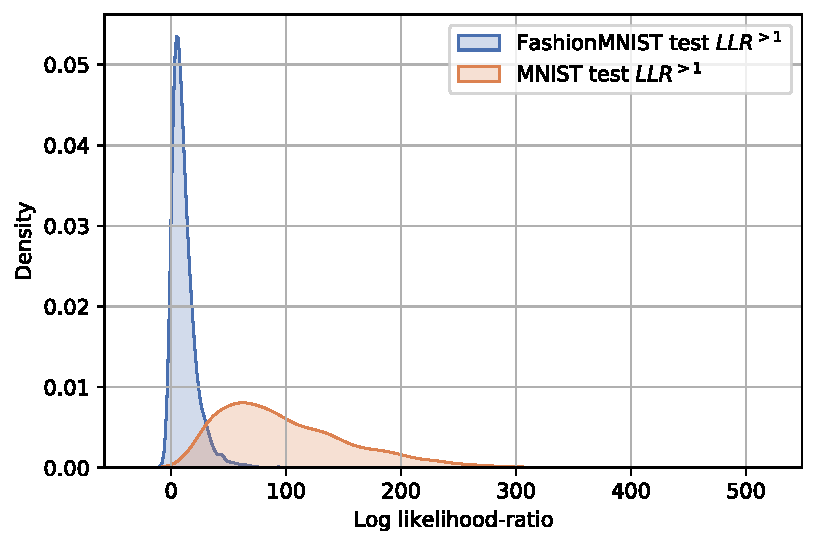
\includegraphics[width=1\columnwidth]{paper_hierarchical/densities-FashionMNIST-test-MNIST-test-LLR-0-1_sohau.pdf}
        \caption{}
        \label{fig_hierarchical:FMNIST-llr}
    \end{subfigure}
    \caption[Empirical densities of FashionMNIST (in-distribution) and MNIST (OOD) using the raw likelihood and $\mathcal{L}^{>2}$ bound.]{%
    Empirical densities of FashionMNIST (in-distribution) and MNIST (OOD) using the raw likelihood \subref{fig_hierarchical:FMNIST-elbo-k0}, the $\mathcal{L}^{>2}$ bound \subref{fig_hierarchical:FMNIST-elbo-k2} and the $LLR^{>1}$ score \subref{fig_hierarchical:FMNIST-llr}. All densities are computed using the HVAE model.
    For the regular likelihood MNIST is very clearly more likely on average than the FashionMNIST test data while with the $\mathcal{L}^{>2}$ bound separation is better but significant overlap remains.
    The $LLR^{>1}$ provides a high degree of separation. Likelihoods are reported in units of the natural log of the number of bits per dimension.
    }
    \label{fig_hierarchical:FMNIST-ood-densities}
\end{figure}
% \end{sidewaysfigure}

We first report the results of the different variations of the $\mathcal{L}^{>k}$ bound for OOD detection. 
We reconfirm the results of \textcite{nalisnick_deep_2019} by observing that our hierarchical latent variable models also assign higher $\mathcal{L}^{>0}$ to the OOD dataset in the FashionMNIST/MNIST and CIFAR10/SVHN cases resulting in an AUROC$\uparrow$ inferior to random (\cref{tab_hierarchical:rocauc-ood}).
Switching the in-distribution data for the OOD data in both cases result in correctly detecting the OOD data; an asymmetry also reported by \textcite{nalisnick_deep_2019}.
\cref{fig_hierarchical:FMNIST-elbo-k0} shows the density of $\mathcal{L}^{>0}$ in bits per dimension \cite{theis_note_2016} by the model trained on FashionMNIST when evaluated on the FashionMNIST and MNIST test sets.
We observe a high degree of overlap, with less separation of the OOD data compared to similar results of autoregressive and flow-based models, like \textcite{xiao_likelihood_2020}.


We then evaluate the looser $\mathcal{L}^{>k}$ \cref{eq_hierarchical:biva->k} for $k\in\{1,L\}$.
\cref{fig_hierarchical:FMNIST-elbo-k2} shows the result for $\mathcal{L}^{>2}$, which yielded the highest AUCROC$\uparrow$, only slightly better than random.
Like \textcite{maaloe_biva_2019}, we see that increasing the value of $k$ generally leads to improved OOD detection.
However, we also observe that the two empirical distributions never cease to overlap.
Importantly, depending on the OOD dataset, the amount of remaining overlap can be high which limits the discriminatory power of the likelihood-based $\mathcal{L}^{>k}$ bound.
This is in-line with the pathological behavior of the raw likelihood of latent variable models when used for OOD detection \cite{xiao_likelihood_2020}.
Since a high degree of overlap also seems present in \textcite{maaloe_biva_2019}, and we see the same problem for our BIVA model trained on CIFAR10, we do not expect this to be due to the less expressive HVAE.


\subsection{Likelihood-ratio-based OOD detection}
\begin{figure}
    \centering
    \begin{subfigure}[l]{0.495\columnwidth}
        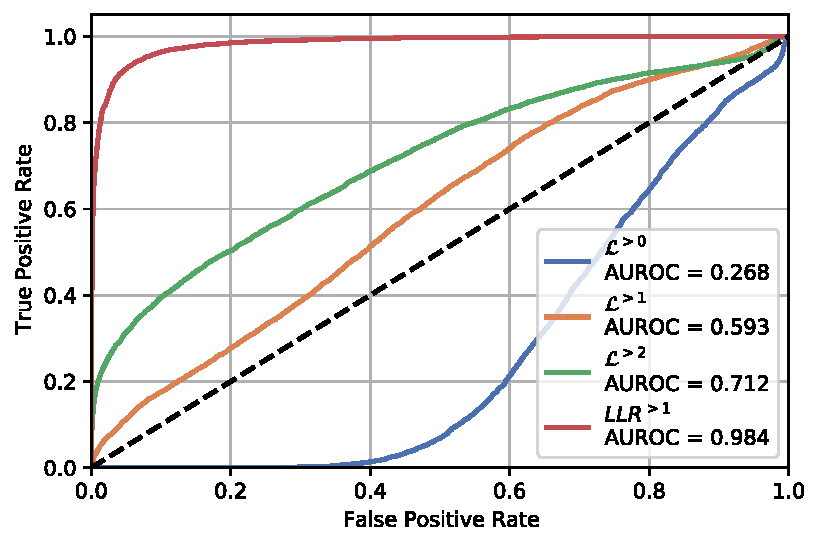
\includegraphics[width=1\columnwidth]{paper_hierarchical/roc-FashionMNIST-test-MNIST-test-ll-and-llr-IW250_sohau.pdf}
        \caption{}
        % \caption{ROC curves with AUROC score for detecting MNIST as OOD with the HVAE model trained on FashionMNIST.
        % A ROC curve is plotted for each of the $\mathcal{L}^{>k}$ bounds including the ELBO along with one for the best-performing log likelihood-ratio $LLR^{>1}$.}
        \label{fig_hierarchical:FMNIST-roc-llr}
    \end{subfigure}
    \hfill
    \begin{subfigure}[r]{0.495\columnwidth}
        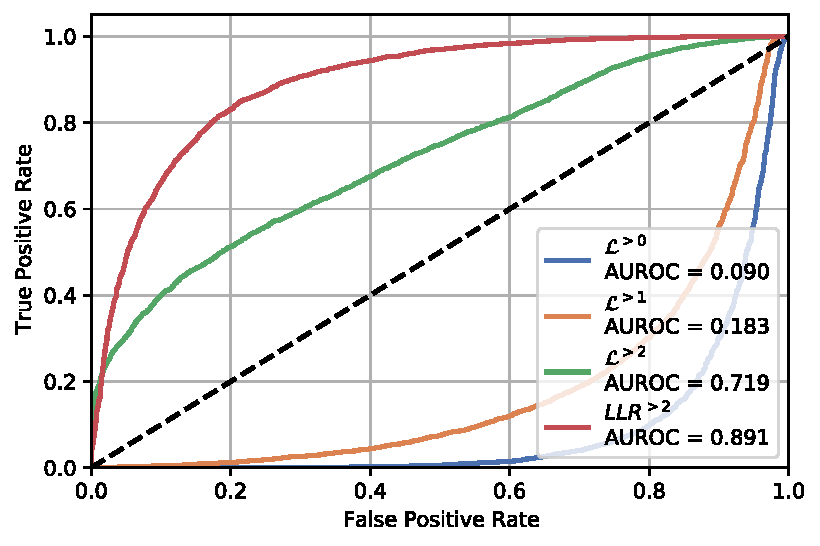
\includegraphics[width=1\columnwidth]{paper_hierarchical/roc-biva-CIFAR10-SVHN-ll-and-llr_sohau.pdf}
        \caption{}
        % \caption{ROC curves with AUROC score for detecting SVHN as OOD with the BIVA model trained on CIFAR10.
        % A ROC curve is plotted for each of the $\mathcal{L}^{>k}$ bounds including the ELBO along with one for the best-performing log likelihood-ratio $LLR^{>2}$.}
        \label{fig_hierarchical:CIFAR10-roc-llr}
    \end{subfigure}
    \caption[ROC curves for out of distribution detection (MNIST/FashionMNIST and SVHN/CIFAR10).]{%
        ROC curves with AUROC score for detecting \subref{fig_hierarchical:FMNIST-roc-llr} MNIST as OOD with the HVAE model trained on FashionMNIST and \subref{fig_hierarchical:CIFAR10-roc-llr} SVHN as OOD with the BIVA model trained on CIFAR10. 
        A ROC curve is plotted for each of the $\mathcal{L}^{>k}$ bounds including the ELBO along with one for the best-performing log likelihood-ratio $LLR^{>1}$.
    }
\end{figure}
We now move to the likelihood ratio-based score.
We find that $LLR^{>k}$ separates the OOD MNIST data from in-distribution FashionMNIST to a higher degree than the likelihood estimates as can be seen by the empirical densities of the score in \cref{fig_hierarchical:FMNIST-llr}.
We note that the likelihood ratio between the ELBO and the $\mathcal{L}^{>k}$ bound provides the highest degree of separation of MNIST and FashionMNIST as measured by the AUROC$\uparrow$ for $k=1$ smaller than $L$.
This is not surprising since the value of $k$ that provides the maximal separation to the reference in-distribution dataset need not be the one for which $\mathcal{LLR}^{>k}$ is overall maximal for the OOD dataset.
We also visualize the ROC curves resulting from using the $LLR^{>k}$ score for OOD detection on both FashionMNIST/MNIST and CIFAR10/SVHN and compare it to the ROC curves resulting from the different $\mathcal{L}^{>k}$ bounds in Figures \ref{fig_hierarchical:FMNIST-roc-llr} and \ref{fig_hierarchical:CIFAR10-roc-llr}, respectively.
On both datasets we see significantly better discriminatory performance when using the $LLR^{>k}$ score.

\cref{tab_hierarchical:rocauc-ood} shows that BIVA improves upon the HVAE model for OOD detection on CIFAR while \cref{tab_hierarchical:bits-per-dim-ood} shows that the BIVA model also improves upon the HVAE in terms of likelihood.
We hypothesize that models larger than our implementation of BIVA, with better likelihood scores may perform even better \cite{maaloe_biva_2019, vahdat_nvae_2020, child_very_2021}.


\subsection{Comparison to baselines}
\paragraph{Performance} \cref{tab_hierarchical:rocauc-ood} summarize our results compared to baselines based on the commonly used AUROC$\uparrow$, AUPRC$\uparrow$ and FPR80$\downarrow$ metrics.
Our method outperforms other generative model-based methods such as WAIC \cite{choi_waic_2019} with Glow model and performs similarly to the likelihood regret method of \cite{xiao_likelihood_2020}.
Furthermore, our method performs similarly to the background constrative likelihood ratio method of \textcite{ren_likelihood_2019} on FashionMNIST/MNIST but contrary to the failure of that method on CIFAR10/SVHN reported by \cite{xiao_likelihood_2020}, our method performs very well on this task too.
Our approach outperforms all supervised approaches that use in-distribution labels or synthetic examples of OOD data derived from the in-distribution data including ODIN \cite{liang_enhancing_2018} and the predictive distribution of a classifier $p(\hat{y}|\xb)$ trained and evaluated in various ways (see \textcite{ren_likelihood_2019}).

\paragraph{Runtime} For a full evaluation of a single example across all feature levels of a model with $L$ stochastic layers, our method requires $L-1$ forward passes through the inference and generative networks as well as computing the likelihood ratio, of which the forward passes are dominant.
For a typical forward pass that is linear in the input dimensionality, $D$, and the number of stochastic layers, $L$, this amounts to computation of $\mathcal{O}(DL)$.
Compared to some related work that either requires an $M>1$ sized batch of inputs of which either all or none are OOD \cite{nalisnick_detecting_2019} or cannot be applied to batches due to the required per-example optimization \cite{xiao_likelihood_2020}, our method additionally is applicable to batches of any size that may consist of both OOD and in-distribution examples which provides drastic speed-ups via vectorization and parallelization.
Furthermore, the method of \textcite{xiao_fashionmnist_2017} requires refitting the inference network of a VAE which can be computationally demanding.
Compared to the likelihood ratio proposed in \textcite{ren_likelihood_2019}, our method requires training only a single model on a single dataset.


\section{Discussion}
Deep generative models are state-of-the-art density estimators, but the OOD failures reported in recent years have raised concerns about the limitations of such density estimates. Recent work on improving OOD detection has largely sidestepped this concern by relying on additional assumptions that strictly should not be needed for models with explicit likelihoods.
While the engineering challenge of building reliable OOD detection schemes is important, it is of more fundamental importance to understand \emph{why} the naive likelihood test fails.
We have provided evidence that low-level features of the neural nets dominate the likelihood, which gives a \emph{cause} to the \emph{why}.
The fact that a simple score for measuring the importance of semantic features yield state-of-the-art results on OOD detection without access to additional information gives validity to our hypothesis.

The findings from, amongst others, \textcite{nalisnick_deep_2019, serra_input_2020} have a clear relation to information theory and compression. 
Semantically complex in-distribution data yields models with diverse low-level feature sets that enable generalization across datasets.
Simpler datasets can only yield models with less diverse low-level feature sets compared to complex training data.
Hence, there can be an asymmetry where the likelihoods of simple OOD data can be high for a model trained on complex data, but not the other way around.
Loosely put, the minimal number of bits required to losslessly compress data sampled from some distribution is the entropy of the generating process \cite{shannon_mathematical_1948, mackay_information_2003}.
\textcite{townsend_practical_2019} recently showed that VAEs can be used for lossless compression at rates superior to more generic algorithms.

We also note that since the hierarchical VAE is a probabilistic graphical latent variable model, it lends itself very naturally to manipulation at the feature level \cite{kingma_semi-supervised_2014, maaloe_auxiliary_2016, maaloe_semi-supervised_2017}.
This property sets it apart from other generative models that do not explicitly define such a hierarchy of features.
This in turn enables reliable OOD detection with our methodology while making no explicit assumptions about the nature of OOD data and only using a single model. This has not been achieved with autoregressive or flow-based models.

\section{Conclusion}
In this paper we study unsupervised out-of-distribution detection using hierarchical variational autoencoders.
We provide evidence that highly generalizeable low-level features contribute greatly to estimated likelihoods resulting in poor OOD detection performance.
We proceed to develop a likelihood-ratio based score for OOD detection and define it to explicitly ensure that data must be in-distribution across all feature levels to be regarded in-distribution.
This ratio is mathematically shown to perform OOD detection in the latent space of the model, removing the reliance on the troublesome input-space likelihood.
We point out that contrary to much recent literature on OOD detection, our approach is fully unsupervised and does not make assumptions about the nature of OOD data.
Finally, we demonstrate state-of-the-art performance on a wide range of OOD failure cases.


\section*{Acknowledgements}
This research was partially funded by the Innovation Fund Denmark via the Industrial PhD Programme (grant no.\@ 0153-00167B). JF and SH were funded in part by the Novo Nordisk Foundation (grant no.\@ NNF20OC0062606) via the Center for Basic Machine Learning Research in Life Science (MLLS, \hyperlink{https://www.mlls.dk}{https://www.mlls.dk}). JF was further funded by the Novo Nordisk Foundation (grant no.\@ NNF20OC0065611) and the Independent Research Fund Denmark (grant no.\@ 9131-00082B). SH was further funded by VILLUM FONDEN (15334) and the European Research Council (ERC) under the European Union’s Horizon 2020 research and innovation programme (grant agreement no. 757360).

% }

% End slide
\frame{\centering\Huge Thank you for your attention}

% Bibliography slide
\begin{frame}[allowframebreaks]{Bibliography}\printbibliography\end{frame}

\end{document}